
\documentclass[master]{thesis-uestc}


\title{基于FPGA的循环神经网络前向传播加速技术研究}{Research 
	on Forward Propagation Acceleration Technology of Recurrent Neural Network Based on FPGA}

\author{杨钦惠}{Yang Qinhui}
\advisor{王海\chinesespace 教授}{Dr. Hai Wang}
\school{集成电路科学与工程学院(示范性微电子学院)}{School of Integrated Circuit Science and 
	Engineering (Examplary School of Microelectronics)}
\major{集成电路工程}{Integrated Circuit Engineering}
\studentnumber{202022021509}
% require all the usepackages here
% \usepackage{algorithm2e}

\begin{document}

\makecover

% This is a template of mutiple files.
% The folders chapters/ and misc/ have the related files

% abstract
	
\begin{chineseabstract}
循环神经网络是一类专门针对序列数据处理任务而设计的神经网络,广泛应用于语音识别,机器翻译和动态系统建模等领域,在时间序列相关的任务上拥有
超越其他神经网络模型的性能表现。随着任务复杂度的增长与人们对模型预测效果需求的提高,循环神经网络的模型参数量也越来越大,这对硬件
实现平台造成了巨大的存储和计算压力,也带来了高延迟等问题,阻碍了循环神经网络在更广阔场景的应用,例如嵌入式场景和IoT场景等。现有的工作分别
从模型压缩算法和硬件加速技术着手,提出了一些经典的解决方案如剪枝算法和硬件加速器,但是这些方案存在压缩成本过高,加速器专用型过强等缺陷,
无法应用在对精度和速度有动态调节需求的场景中,而这类场景又是普遍存在的。因此,开发具备精度速度动态调节能力的循环神经网络加速技术存在
很大的实用价值。

%忽视了应用场景的需求。
%因此尽管一些应用场景和需求是普遍存在的,例如具有弹性需求的场景,现有的方案由于压缩成本过高,加速器专用性过强等缺陷无法高效的完成这些工作。
针对上述问题,本文研究了循环神经网络前向前向传播过程的加速技术,基于FPGA设计并实现了具备精度和速度调节能力的循环神经网络加速系统。该系统借助基于投影的压缩算法的低成本优势,并将其和
网络的前向传播过程有机结合,实现了在系统运行过程中生成并切换到指定网络尺寸的功能,最终达成了调节系统精度速度的目的。首先,本文进行了系统架构
分析与设计,将系统的各功能组件映射到具体的软硬件实现,合理的功能划分使得系统能够高效的运转。其次,在软件算法设计上,本文考虑了系统在实际
运行过程中可能存在的突发情况,提出了基于预置投影矩阵的方法和基于状态采样的方法,这两种模型生成方法分别对应着普通应用场景和异常状态场景。
充分的应用场景考虑使得系统拥有了环境的鲁棒性。然后,在硬件实现方面,本文设计了加速循环神经网络前向传播过程的硬件加速器,
该加速器能够运行两种不同结构的网络模型并且能调节网络的尺寸,动态可调功能的硬件基础是基于分块矩阵向量乘法的计算模块。
最后,本文对系统消耗的资源进行优化,主要是使用分段三次函数近似方法优化了激活函数模块的资源消耗。系统运行效果的实验表明本文设计实现的
循环神经网络加速系统具备精度和速度的动态调节能力,加速器性能测试实验表明本文的加速器资源消耗较为合理。


%针对上述问题,本文在应用场景弹性需求的驱动以及现实资源有限的束下,以加速循环神经网络的前向传播过程为研究目标,提出了一套从算法,软件,硬件
%再到系统集成的完整解决方案。该方案通过调节网络尺寸满足了用户对模型预测精度和速度的弹性需求,通过软硬件划分实现了系统各功能组件的高效
%运转,通过定制专用硬件架构获得了网络前向传播过程计算性能的提升。首先,本文使用了基于投影方法的模型压缩算法以降低循环神经网络的模型参数量,
%包括状态近似和激活函数近似,该模型压缩算法具有压缩成本低,无需训练集以及精度损失小等优势。其次,考虑到压缩算法的低成本特性以及模型尺寸
%对网络前向传播速度的影响,本文设计了循环神经网络加速系统,该系统将网络的压缩过程和前向传播过程有机结合,
%在运行过程中可根据用户和环境对速度和精度的需求运行压缩算法生成特定尺寸的网络模型并以该尺寸模型进行前向传播。
%最后,系统的具体实现由软硬件分工协同完成。在软件方面,%根据压缩算法的数据来源不同,
%本文提出了两种压缩流程,分别是基于预置投影矩阵的方法和
%基于状态采样的方法,这两种方法对应着普通场景和异常状态场景。在硬件方面,本文设计了循环神经网络加速器,加速器主要由矩阵向量并行乘法模块和
%分段近似激活函数模块组成,并且在架构设计层面使用了模块共享和分时复用技术,有效的节省了硬件资源消耗。本文的设计基于FPGA完成实现与验证,
%实验表明本文所设计的系统能够实现模型压缩,网络模型切换和调节模型尺寸等功能,满足场景对循环神经网络前向传播速度和精度的弹性需求。



\chinesekeyword{循环神经网络,回声状态网络,硬件加速器,FPGA,高层次综合}
\end{chineseabstract}



\begin{englishabstract}
Recurrent Neural Networks (RNNs) are a type of neural network designed specifically for processing sequential data, 
and are widely used in various fields such as speech recognition, machine translation, and dynamic system modeling. 
RNNs have shown superior performance compared to other neural networks in time sequences related tasks.
With the increasing complexity of tasks and demanding for better model prediction accuracy, the parameter size of 
Recurrent Neural Networks (RNNs) has also become larger, which resulting 
in significant storage and computational pressure on hardware implementation platforms and also lead to the high latency problem. 
Those problems hinder the wider application of RNNs in various scenarios, such as embedded system and IoT environments.
Existing work has proposed some classical solutions, such as pruning algorithms and hardware accelerators, focusing on 
model compression and hardware acceleration techniques. 
However, these solutions have great shortcomings such as high compression costs and strong accelerator specialization, 
making them unsuitable for scenarios requiring dynamic adjustment of accuracy and speed, which are commonly encountered. 
Therefore, there is significant practical value in developing Recurrent Neural Network (RNN) acceleration technologies with 
the ability to dynamically adjust precision and speed.

To solve the above problems, this thesis designs and implements an RNN acceleration system with adjustable precision and 
speed based on FPGA. 
This system leverages the low-cost advantage of projection-based compression algorithm and organically integrates it with 
the forward propagation process of the network to generate and switch to specified network sizes during system running,
ultimately achieving the goal of adjusting the system's accuracy and speed. 
Firstly, this thesis analyzed and designed the system architecture, and mapped each function component to specific software 
and hardware implementations. The rational partitioning enables the system to operate efficiently.
Secondly, in terms of software algorithm design, this thesis considers possible emergent situations during system operation 
and proposes methods based on pre-set projection matrices method and state sampling method, respectively corresponding to 
normal state scenarios and abnormal state scenarios. 
Sufficient consideration of various scenarios enhances the system's robustness in different environments.
Thirdly, in terms of hardware implementation, this thesis designed a hardware accelerator to accelerate the forward propagation 
process of recurrent neural networks. The accelerator can run two different network models and adjust the model's size, 
Dynamic adjustability is achieved from the blocked matrix-vector multiplication.
Finally, this thesis optimizes the resource consumption of the system by using a segmented cubic function approximation method to 
optimize the resource consumption of the activation function module.
Experimental results on the system performance show that the designed and implemented recurrent neural network acceleration system 
in this thesis has dynamic adjustability of accuracy and speed. Performance testing experiments on the accelerator indicate that
the resource consumption of this accelerator is reasonable.

\englishkeyword{Recurrent Neural NetWorks, Echo State Networks, Hardware Accelerator, FPGA, High-Level Synthesis}
\end{englishabstract}


% table of contents
\thesistableofcontents

% thesis contents
\chapter{绪\hspace{6pt}论}

\section{研究背景与意义}
人工智能(Artificial Intelligence,AI)自上世纪五十年代诞生以来,经过符号主义,联结主义,行为主义三大流派的发展,理论和技术取得了长足的进步。
近年来,基础算力的提升和大数据的兴起促使了人工智能新一轮的应用浪潮。
智能算法在语音语言,图像视频,推荐搜索,自动驾驶等领域都取得了革命性突破。
其中以深度神经网络为代表的算法相较传统算法表现出更优越的性能,在面对与日俱增的精度需求和纷繁复杂的任务场景时都能保持较好的学习和预测能力。

神经网络算法包含众多模型,其中广泛应用的网络包括前馈神经网络(feedforward neural network, FNN),循环神经网络(recurrent neural network, RNN),
卷积神经网络(convolutonal neural network, CNN),生成对抗深经网络(generative adversarial network,GAN)等。这些网络模型及其组合变体可针对性
的解决不同应用场景的任务需求。理论而言,只要数据集足够完备,模型规模足够大,神经网络可以作为万能近似器以任意精度逼近复杂函数\citing{Hornik}。
实际情况也正如此,为达到更高的精度和获得更好的模型泛化能力,神经网络朝着深层,大参数,高计算量和复杂结构的方向发展。
自2017年提出了基于注意力机制的Transformer网络结构后,基于Transformer网络的GPT (Generative Pre-trained Transformer) 系列模型参数量从GPT-1的亿级,
增长到到GPT-2的十亿级,再到最新的ChatGPT的千亿级,网络模型参数量随时间呈指数级增长。

然而在硬件方面,由于登纳德缩放定律(Denard Scaling)以及摩尔定律( Moore‘s Law)的停滞,通用处理器性能提升速度明显放缓。CPU频率和晶体管
密度难以持续增长,体系结构优化空间接近上限,多核性能受到带宽和功耗的限制,通用处理器的单位性能提升的成本也越来越大。1986年至2003年通用处理器
性能每年提升约50\%,符合摩尔定律的预测,但近10年来其性能增速明显放缓\citing{ComputerArchi}。后摩尔定律时代,领域
专用架构(Domain Specific Architecture,DSA)是一种继续为上层应用提供高性能算力的解决方案,也是近年来的趋势。领域专用架构针对应用和算法
的特性定制指令和微架构,充分利用每一个晶体管,设计实现专用硬件加速器,以牺牲通用性为代价换取特定应用领域的高性能和高能效。近年来,GPU,
FPGA,ASIC等定制化硬件加速器在数据中心和边缘设备得到大规模部署,为大数据时代提供了强大的算力支撑。针对蓬勃发展的人工智能应用,研究人员
根据不同的神经网络结构定制化的提出了适应其特性的专用加速器,获得了比通用处理器更高的性能。

综上所述,人工智能应用的蓬勃发展和硬件算力的停滞不前是当下不容忽视的矛盾。这组矛盾一方面阻碍了神经网络朝着大模型,大数据,多任务
的发展趋势,另一方面也阻碍了工业界对成熟人工智能应用的落地与普及。提升算力,设计专用加速器,为算法和模型的再次进步提供强有力的支撑
已成为迫切的需求以及研究的热点。

本文选取循环神经网络作为研究对象,目的是设计专用硬件加速器以满足一类普遍应用场景的需求,达到功耗,延迟以及精度等方面性能的平衡与提升。
循环神经网络是一类用于处理序列数据的神经网络模型,广泛应用于语音识别,机器翻译和动态系统建模,在涉及时间序列相关的应用上表现出超越其他
网络模型的性能。通过向网络结构中引入反馈机制,循环神经网络一方面可以在时间维度上共享参数,做到学习不同长度样本的经验并进行泛化;另一方面,
隐藏单元作为过去信息的有损摘要可以巧妙的实现记忆和遗忘功能,从而捕获输入数据的长期依赖关系。为了获得更好的模型预测效果,循环神经网络
往往包含大量隐藏层单元,其状态的更新来自于仿射变换(矩阵向量乘法)和紧随其后的非线性变换(激活函数)。从计算的角度,这些变换是循环神经
网络中计算最密集的部分,也是循环神经网络推理最耗时的部分,计算带来的高延迟会影响交互式应用场景下的用户体验。从存储的角度,随着循环神经
网络模型规模的增长,其所需要存储的参数量呈平方增长,这将导致循环神经网络难以部署在存储资源有限的终端设备如嵌入式设备和移动设备。
从功耗的角度,IoT和端侧人工智能有严格的能源预算要求,现有的神经网络实现平台如CPU和GPU因能源消耗大不适宜在边缘场景应用。
从用户需求求角度,用户对神经网络模型预测精度,功耗和速度的需求并非一成不变,任务的到达时间可能密集亦或稀疏,任务的目的可能是识别
或者只需要判断。面对多样化的用户需求,算法和硬件需要具备弹性可伸缩的特性。

针对以上问题,现阶段的解决方案包括软件算法端减少算力需求,硬件端增加算力提供,软硬件协同设计。本文对现有的解决方案进行综合考虑,针对
具有弹性需求的应用场景提出一套从算法,软件到硬件的解决方案及设计流程。该方案采用压缩算法对循环神经网络模型进行压缩,在硬件端设计专用
加速器实现性能提升。考虑到压缩算法将原始网络压缩为精简网络的过程不需要基于训练集的反向传播(无数据集和低压缩成本特性),网络模型的
压缩过程可以在终端设备实现。这使得终端设备在无云端支持的条件下能够独立且完备的运行,并且可以根据应用场景的具体需求以合适的网络大小
运行。在硬件层面FPGA具有可重构,高并行,低功耗的特性,一方面可以快速迭代设计高效的专用硬件架构,另一方面又可以模拟资源有限的边缘应用场景,
是实现循环神经网络硬件加速器设计的理想平台。此外,软硬件协同也是循环神经网络成为完整产品的必要环节,在任务目的,功耗,资源和实现成本等
条件的约束下,本文采用合适的软硬件划分与协同以高效完成设计目标。本文无法为所有的应用和算法设计实现硬件加速方案,仅针对循环神经网络的模型压缩
和硬件加速进行研究和实践,希望能为未来的研究提供借鉴和参考。

%一会儿任务密集,需要高精度,一会儿,任务稀疏,需要低功耗,满足这类需求是必要的,因此需要自适应的变换尺寸。

%数学语言描述为输出的每一项是对先前的输出应用相同规则而产生。也正因为此,当网络需要学习长期依赖关系的信息时,基于梯度的优化会变得困难。
%研究表明,SGD在依赖关系跨度为10到20的序列上完成训练的可能性为0\citing{Bengio1994b},具体表现为梯度消失和梯度爆炸问题\citing{Hochreiter}。 
%为解决该问题,研究人员一方面设计新的网络结构,长短期记忆网络(Long short-term Memory,LSTM),门控循环单元(Gate recurrent unit,GRU)
%和回声状态网络(Echo state network,ESN)基于此背景提出,另一方面通过增加隐藏层单元数量以增强模型记忆能力。

\section{国内外研究现状}
人工智能产业有广阔的市场前景和经济价值,但应用的研究和实际落地还存在一定距离,主要体现在模型规模越来越大和硬件资源有限这一冲突。研究人员
从神经网络压缩算法和硬件加速器设计两方面尝试给出解决方案。
\subsection{神经网络压缩算法研究现}
研究表明神经网络中存在大量的冗余性,包括结构冗余和参数冗余。神经网络架构搜索(Neural Architecture Search, NAS)是一种自动搜索并优化神经
网络架构的技术\citing{NAS_ICLR, NAS_CVPR},其在候选神经网络结构的集合中通过某种策略搜索出最优网络结构。例如MobileNet\citing{MobileNetsV1,MoileNetsV2},
ShuffleNet\citing{Shuffnet},SqueezeNet\citing{}等在不损失模型准确率的条件下具有更加紧凑的模型结构。LSTM网络结构中遗忘门是最重要的结构,
输入门次之,输出门影响最小\citing{CompRNN},GRU,MGU,S-LSTM以及JANET对LSTM模型中的门控单元进行简化,降低了网络的结构复杂度。

剪枝是应用最广泛的网络模型参数压缩方法,主要可以分为神经元剪枝和权重剪枝。前者减少神经网络中的节点数量,后者减少神经网络中的连接数量。
剪枝方法最早在上世纪90年代的论文\citing{Purning}中提出,在2015年,Han等人对剪枝方法进行改,以较小的幅度修剪权重和神经元以降低CNN
前向传播的计算复杂度\citing{WeightPurning},并且其所提出的Train-Purne-Retrain的剪枝方法能解决剪枝后模型精度下降的问题,广泛的应用于
后续的基于剪枝的模型压缩工作中。这种对每一个权重值进行细颗粒度的剪枝方法方法尽管能够有效减少模型参数量,但却引入了对硬件
不友好计算和访存模式,即非零数据的不规则分布会带来无效的数据计算以及流水线的阻塞。ESE\citing{ESE}是一种负载均衡的剪枝方法,该方法在
剪除小权重的同时保证分配到每一个运算处理单元的计算量相当,最终相较稠密的LSTM,压缩后的模型达到了90\%的压缩比和6.2倍的加速比。C-LSTM\citing{C-LSTM}
采用结构化的剪枝方法,以二维矩阵块为剪枝粒度,剪枝后的权重消除了计算的不平衡性。文献以CNN中的Kernel,Filter,Channel为剪枝对象,同样
增加了剪枝粒度,在极大减小模型参数的同时又保持了对硬件执行友好的特性。粗颗粒剪枝具有压缩率高,数据结构规则等优势,但同时也面临着模型
准确率下降的问题,Cao\citing{Cao}提出了基于组平衡稀疏的剪枝方法,在矩阵块间保持计算平衡的基础上对每一块内部采用细颗粒的权重剪枝,提高了模型的准确率。
AutoMl\citing{AutoMl1,AutoMl2}等自动优化方法将剪枝定义为一个优化问题,能够以较高的精度自动搜索最佳的剪枝位置和比例。

\subsection{神经网络硬件加速平台研究现状}

\section{本文的主要研究内容}
本论文以时域积分方程时间步进算法的数值实现技术、后时稳定性问题以及两层平面波加速算法为重点研究内容,主要创新点与贡献如下:

\section{本论的结构安排}
本文的章节结构安排如下:
网络模型的性能。通过向网络结构中引入反馈机制,循环神经网络可以在时间维度上共享参数,。

\chapter{循环神经网络加速技术基础}

\section{循环神经网络及其变体}
循环神经网络是一种专门针对序列数据进行建模的神经网络模型。有别于前馈神经网络,卷积神经网络等“静态模型”,循环神经网络在结构上拥有循环
自连接的反馈机制,这使得模型当前的输出不仅取决于当前输入,还与当前的状态有关。通过对状态的存储与更新,循环神经网络能够有效的建模动态系统。
理论上,任何图灵可计算的函数都可以用有限维的循环网络近似。尽管循环神经网络功能强大,但是高昂的训练成本阻碍了循环神经网络的实际应用。
一方面,固定有序的前向传播过程只能遵循序列顺序先后计算,因此通过时间的反向传播无法并行计算;另一方面,梯度消失和梯度爆炸问题在循环神经网络
的训练过程中尤为突出,这导致其学习长期依赖关系变的困难。随着理论研究的发展和算力的提升,以上问题都得以解决。借助第三次人工智能浪潮
循环神经网络重新焕发出勃勃生机,目前,循环神经网络已经广泛应用于自然语言处理等相关领域。

\subsection{普通循环神经网络}
普通循环神经网络是最简单的循环神经网络结构,主要包括输入层,隐藏层和输出层。输入层对输入进行特征提取并映射为固定长度的向量,隐藏层将输入信息
和前一时刻的状态转化为新的状态,输出层根据网络存储的状态解码并完成输出。其中隐藏层包含记忆信息以及记忆更新的规则,是循环神经网络中最重要的
结构。
常见的循环神经网络结构如图\ref{fig:rnn}所示,权重矩阵\(U, W, V\)分别表示输入到到隐藏,隐藏到隐藏,隐藏到输出之间的连接,向量\(x, h, o\)分别表示输入单元,
隐藏单元和输出单元,这些单元及其相互连接形成网络。相比于其他网络模型的单向信息传递,循环神经网络引入环状结构实现了从输入到输出的双向信息
流动。一些符合训练准则的信息将会通过循环的方式长期保存在网络状态中,并根据输入序列特征进行适时唤醒记忆。当网络记忆的信息足够丰富时,循环神经
网络不仅能准确的预测输出,并且能大致恢复输入序列。自编码器框架就是基于此原理而产生,其能根据记忆的状态信息选择重要的输入并近似复制到输出,
实现特征学习或降维。图中左侧为循环神经网络回路原理图,黑色方块表示回路中单个时间步的延迟,即时刻t-1的状态会影响时刻t的状态。图中右侧为
循环神经网络按时间展开的计算图,展开是指将左侧的回路结构映射为右侧的包含重复组件的结构,展开的深度取决与序列的长度。循环神经网络展开结构图
显式的数据流动路径描述了信息是如何在时间上向前和向后传递的。
\begin{figure}
	\centering
	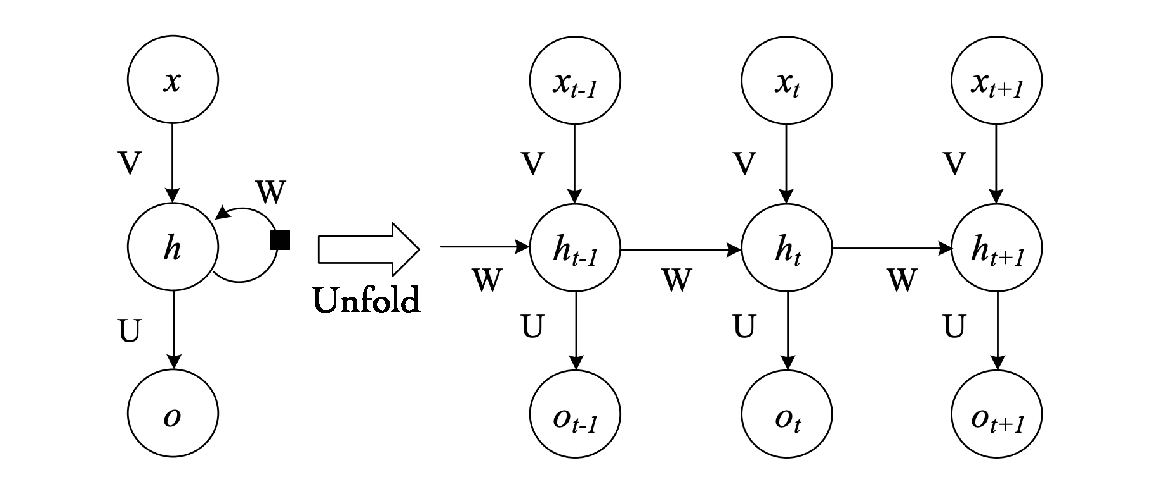
\includegraphics[width=0.8\columnwidth]{RNN_struct.eps}
	\caption{循化神经网络结构图}
	\label{fig:rnn}
\end{figure}

循环神经网络的数学模型为式\ref{eq:rnn},

\begin{equation}\label{eq:rnn}
	\begin{split}
		h_{t} &= g(W*h_{t-1} + U*x_{t})	\\
		y_{t} &= f(V*h_{t})						
	\end{split}
\end{equation}





\begin{align*}
&i_t = \sigma(W_{ix}*x_t + W_{ir}*y_{t-1} + W_{ic}*c_{t-1} +b_i)	\\
&f_t = \sigma(W_{fx}*x_t + W_{fr}*y_{t-1} + W_{fc}*c_{t-1} +b_f)	\\
&g_t = \sigma(W_{cx}*x_t + W_{cr}*y_{t-1} + b_c)					\\
&c_t = f_t \odot c_{t-1} + g_t \odot i_t							\\
&o_t = \sigma(W_{ox*x_{t} + W_{or} \*y_{t-1} + W_{oc}*c_t} + b_o)	\\
&m_t = o_t \odot h_{c_t}											\\
&y_t = W_{ym}*m_t													\label{eq:Maxwell}
\end{align*}










\subsection{长短期记忆神经网络}
\subsection{回声状态网络} 

\section{模型压缩与加速算法}
RWG 基函数是定义在三角形单元上的最具代表性的基函数。它的具体定义如下:
\begin{equation}
f_n(\bm{r})=
\begin{cases}
\frac{l_n}{2A_n^+}\bm{\rho}_n^+=\frac{l_n}{2A_n^+}(\bm{r}-\bm{r}_+)&\bm{r}\in T_n^+\\
\frac{l_n}{2A_n^-}\bm{\rho}_n^-=\frac{l_n}{2A_n^-}(\bm{r}_--\bm{r})&\bm{r}\in T_n^-\\
0&\text{otherwise}
\end{cases}
\end{equation}

其中,$l_n$为三角形单元$T_n^+$和$T_n^-$公共边的长度,$A_n^+$和$A_n^-$分别为三角形单元$T_n^+$和$T_n^-$的面积(如图\ref{pica}所示)。

\begin{figure}[h]
	\includegraphics{pica.pdf}
	\caption{RWG 基函数几何参数示意图}
	\label{pica}
\end{figure}

由于时域混合场积分方程是时域电场积分方程与时域磁场积分方程的线性组合,因此时域混合场积分方程时间步进算法的阻抗矩阵特征与时域电场积分方程时间步进算法的阻抗矩阵特征相同。
\begin{equation}
\label{latent_binary_variable}
\bm{r}_{i,j}=
\begin{cases}
1,f(\bm{x}^{i};\bm{w})\cdot f(\bm{x}^{j};\bm{w})\geq u(\lambda),\\
0,f(\bm{x}^{i};\bm{w})\cdot f(\bm{x}^{j};\bm{w})< l(\lambda), 1\leq i,j\leq n.\\
f(\bm{x}^{i};\bm{w})\cdot f(\bm{x}^{j};\bm{w}),\text{otherwise},
\end{cases}
\end{equation}

时域积分方程时间步进算法的阻抗元素直接影响算法的后时稳定性,因此阻抗元素的计算是算法的关键之一,采用精度高效的方法计算时域阻抗元素是时域积分方程时间步进算法研究的重点之一。


\subsection{轻量化网络}

\subsection{模型稀疏化}

\subsection{数值量化}

\subsection{张量分解}

\section{硬件加速平台介绍}

\subsection{FPGA硬件加速技术}

\subsection{开发工具}


如图\ref{picb}和图\ref{picc}所示分别给出了参数$E_0=\hat{x}$,$a_n=-\hat{z}$,$f_0=250MHz$,$f_w=50MHz$,$t_w=4.2\sigma$时,调制高斯脉冲的时域与频域归一化波形图。

\begin{figure}[h]
\subfloat[]{
	\label{picb}
	\includegraphics[width=7.3cm]{picb.pdf}
}
\subfloat[]{
	\label{picc}
	\includegraphics[width=6.41cm]{picc.pdf}
}
\caption{调制高斯脉冲时域与频率波形,时域阻抗元素的存储技术也是时间步进算法并行化的关键技术之一。(a)调制高斯脉冲信号的时域波形;(b)调制高斯脉冲信号的频域波形}
\label{fig1}
\end{figure}

时域阻抗元素的存储技术\citing{xiao2012yi}也是时间步进算法并行化的关键技术之一,采用合适的阻抗元素存储方式可以很大的提高并行时间步进算法的计算效率。

\section{本章小结}
本章首先从时域麦克斯韦方程组出发推导得到了时域电场、磁场以及混合场积分方程。


\chapter{算法分析及系统架构设计}
本章将针对循环神经网络前向传播过程提出一套从软件算法,硬件实现到系统集成的全流程设计框架和独立整的解决方案。不同于所有过往的压缩加速设计,
本文所采用的压缩算法具有压缩成本小,无需训练集等优势,可以不依赖云端算力支持,仅在分布式的边缘设备实现,算法的详细介绍将在3.1节展开。算法特性
决定了其适用场景,而具有弹性性能需求的应用场景又是普遍存在的,所以在现实条件的约束下,本文对算法进行了合理的拆分与协同并分别映射到软件和硬件上
进行执行,具体的系统架构设计见3.2节。最后,面向算法和应用场景需求,本文进行了定制化专用硬件架构的设计,通过对上层应用的需求和硬件加速空间
进行分析,本文创造性的提出了一种具有紧凑计算结构和可配置功能模块的循环神经网络前向传播硬件加速器。该加速器能通过简单的配置和数据重载完成不同网络结构
和不同模型大小的切换,相比传统的神经网络加速器的一种硬件实现对应唯一的网络结构和模型尺寸,本文所设计的加速器即具有“专用”所带来的高效性,
又具有一定程度“通用”所带来的灵活性,能满足弹性应用场景下性能可调的需求。在众多的循环神经网络模型中,本文选取回声状态网络作为设计实例,因其结构简单,
训练成本低和应用前景开阔等优势,同时又极具代表性和紧迫性,详细分析说明可见2.1节。对于其他种类的循环神经网络,除具体实现细节存在微小差异外,本文在
系统层面提出的设计方案,软件算法和硬件架构设计也同样适用,因此,本文不再一一说明。
\section{基于投影的模型压缩算法}
本小节先展示模型压缩的效果---简化网络结构,然后就简化网络的生成过程(状态投影和激活函数近似)作详细的说明,最后会评估与分析压缩算法的特性和作用效果。
以上描述的模型压缩的全景图是本文后续工作的基础。
\subsection{简化网络结构}
回声状态网络在模型压缩算法的作用下生成了简化网络,其数学模型为式\ref{eq:redesn},式中\(\widehat{x},\widehat{z} \in \mathbb{R}^q\)表示简化网络隐藏层的状态,
\(\widehat{W}, \widehat{E}_d \in \mathbb{R}^{q \times q}\)表示隐藏层与隐藏层的连接权重,\(\widehat{E}_l,\in \mathbb{R}^{q \times q}\)表示隐藏层跨时间步的自循环矩阵,
\(\widehat{W}_{in},\widehat{W}_{out}\in \mathbb{R}^{q \times n_{in}}\)分别表示输入到隐藏层以及隐藏层到输出的连接权重,\(q\)是隐藏层的神经元数量,
\(n_{in}\)为输入数量,\(n_{out}\)为输出数量。
\begin{equation}\label{eq:redesn}
	\begin{split}
		\widehat{z}_t &= f(\widehat{W} * \widehat{x}_{t-1} + \widehat{W}_{in} * u_{t})				\\	
		\widehat{x}_t &= \widehat{E}_l * \widehat{x}_{t-1} + \widehat{E}_d * \widehat{z}_{t} 		\\
		y_{t} 			&= \widehat{W}_{out} * \widehat{x}_{t}	
	\end{split}
\end{equation}

相较于回声状态网络的原网络模型,简化网络的数学描述更加复杂, 具体表现为引入了新的状态变量\(\widehat{z}\)和新的新的拓扑连接\(\widehat{E}_l,\widehat{E}_d\)。
\(\widehat{z}\)是输入\(u\)和状态\(\widehat{x}\)的函数,而\(\widehat{x}\)又与暂态\(\widehat{z}\)呈线性相关的关系。这些新引入的变量和关系
改变了回声状态网络的模型结构,即简化网络在原网络结构的基础上增加了一层隐藏层,如图\ref{fig:esn_convert}所示。此外,简化网络拥有两个循环结构:暂态\(\widehat{z}\)
和状态\(\widehat{x}\)之间的层间循环体和状态层\(\widehat{x}\)内部的自循环体。循环体的增加赋予了循环神经网络更强大的记忆能力,这使得少量的隐藏层神经元
就可以实现对系统动态特性的表征。显然,本文所采用的模型压缩算法在网络结构上做出了让步,但是“祸兮,福之所倚”,简化网络在压缩神经元数量方面取得了巨大的成功。
二者利害相权的最终结果是:在模型预测精度不显著下降的情况下,简化网络的参数量将大幅减少,前向传播过程的时间复杂度也显著降低。
\begin{figure}
	\centering
	\includegraphics[width=0.7\columnwidth]{ESN_convert.eps}
	\caption{原始网络和简化网络的结构图}
	\label{fig:esn_convert}
\end{figure}

简化回声状态网络的结构如图\ref{fig:esn_red}所示。该网络的深度为四,包括输入层\(u\),输出层\(y\)和两层隐藏层\(\widehat{z},\widehat{x}\)。
其中输入层,输出层和状态层\(\widehat{x}\)保留了原网络相似的结构和映射关系。暂态\(\widehat{z}\)是新引入的结构,其作用在于桥接输入层和状态层,
对流经该层的信息做初步的加工处理。暂态层\(\widehat{z}\)和状态层\(\widehat{x}\)共同组成隐藏层,数据在两层隐藏层之间双向流动,形成一个大的信息回路。
但是两层隐藏层也存在差异,暂态层不存在自循环体,因此传统上意义上不能称为状态,考虑到其也位于数据循环的关键路径,因此称之为暂态。实际上
仅从结构特性而言,暂态层和全连接层有更大的相似度。以上分析了简化网络的结构特性,相较于原网络,既存在保留部分,也添加了新的元素。 

\begin{figure}
	\centering
	\includegraphics[width=0.7\columnwidth]{ESN_red.eps}
	\caption{简化回声状态网络结构}
	\label{fig:esn_red}
\end{figure}

简化网络的前向传播速度相较原网络会大幅提升,这得益于隐藏层神经元数量的减少。简化网络内部神经元的数量每层\(q\)个,远小于原网络的\(n\)个。
相应的,网络中神经元的连接复杂度也将降低,权重矩阵的参数量将从\(n^2\)变为\(q^2\)。以上神经元数量和权重参数量的压缩将会直观的反映到模型的
计算复杂度上,原网络每个时间步长的前向传播计算复杂度为
\begin{equation}
	\mathcal{O}(n^2 + n*n_{in} + n*n_{out})
\end{equation}
简化网络的前向传播计算复杂度为
\begin{equation}
	\mathcal{O}(q^2 + q*n_{in} + q*n_{out})
\end{equation}
在输入输出数量不变的条件下,简化网络的时间复杂度仅由\(q\)决定,和原网络的阶数\(n\)无关。又因为\(q<<n\),所以简化网络前向传播的速度会比原网络快很多。
具体的\(q\)值的选取需根据用户对精度和速度的需求来确定,简化网络的阶数\(q\)越小,模型的计算速度越快;\(q\)越大,模型的精度越高。

\subsection{网络压缩}
前面的叙述介绍了简化回声状态网络和原网络之间在网络结构上的相似性和差异性,解释了简化网络模型预测精度不会显著下降的原因,并从计算复杂度的角度说明了
简化网络在前向传播过程中加速能力的来源,下面本小节将就原网络如何生成简化网络进行简要的说明,模型压缩算法的具体推导请见文献\citing{WangLong:TNNLS'23}。
%介绍高速回声状态网络的生成,算法顺序介绍,or硬件需求倒推
\subsubsection{状态近似}
为了记忆动态系统丰富的时序特性,循环神经网络一般拥有庞大数量的隐藏层神经元,这些神经元互连关系复杂,对信息拥有记忆和遗忘功能,是循环神经
网络最重要的组成部分。对于简单的任务,仅需要少量的神经元便可完成,而复杂的任务则需要更多神经元协同。实际情况下,任务的复杂程度判别具有
相当程度的主观性,隐藏层神经元数量会被保守的设置为远超实际需求的数量,即存在大量的冗余性。本小节针对神经元的冗余性,采用基于投影的状态近似方法进行消除。
状态近似框架:
\begin{equation}
	V_x * \widehat{x}_{t} \approx x_{t}
\end{equation}
其中\(V_x \in \mathbb{R}^{n \times q}\)是状态投影矩阵,满足\(V_x^T * V_x = I\),\(x_{t} \in \mathbb{R}^n\)是状态向量,\(\widehat{x}_t \in \mathbb{R}^q\)是状态近似向量。
状态近似将高维向量\(x_t\)投影到状态空间中,并用状态空间的基向量进行线性表示,其坐标为\(\widehat{x}\)。实际上,由于输出只需要选择性的保留
动态系统过去序列的某些方面信息,而与其他方面无关,系统的动态特征往往有限且集中。这在状态空间上表现为:和任务输入输出相关的状态只占全部状态的一部分,即
有效状态空间是满状态空间的子空间。按照状态子空间中特征的重要程度划分,有效状态空间又可以分为核心特性空间和外围特征空间。在进行状态投影时,状态向量将首先
被投影到核心特征空间中,在这种状态近似情况下,模型的预测不会偏离真实输出太大;其次,状态将会被投影到外围特征空间,该空间越大,模型就越能捕捉系统微小
的动态特征,模型的输出也就越具有丰富性。状态子空间的选取将会对状态近似后的网络预测效果产生较大的影响,如何构造状态空间以实现较好的近似将在3.1.2.3中介绍。\\
将状态近似代入回声状态网络模型\ref{eq:esn}得到
\begin{equation}
	\begin{split}
		\widehat{x}_{t} & = V_x^T * f(W*V_x * \widehat{x}_{t-1} + W_{in} * u_t)	\\
					y_t & = W_{out} *V_x * \widehat{x}_t
	\end{split}
\end{equation}
基于投影的状态近似方法生成的简化网络除了隐藏层神经元数量更少以外,还在自循环结构上增加了线性算子。该算子需要在状态激活后
作用于每一个隐藏层神经元,并且运算次数为\(n\),这导致隐藏层的等效神经元数量也为\(n\)。为了获取真正的模型简化,一个直观的想法是将\(V_x^T\)
移动到激活函数内部,形成类似\(V_x^T * W * V_x\)的\(q \times q\)矩阵,这样模型压缩后等效神经元的数量也为\(q\),简化网络前向传播的时间复杂度
也将进一步降低。然而循环神经网络的激活函数通常是非线性的,非线性算子和线性算子的执行顺序是不能更改的,因此此想法无法直接实现。

如果存在矩阵\(P \in \mathbb{R}^{n \times q}\) 能够和非线性运算交换顺序,即矩阵能够穿透激活函数,使得
\begin{equation}
	P^T*f(W*V_x *\widehat{x}_t + W_{in} *u_t) = f(P^T*W*V_x*\widehat{x}_t + P^T *W_{in}* u_t)	
\end{equation}
那么将会实现回声状态网络真正的简化,其模型大小就完全不受原网络尺寸的影响。如何构造这样一个理想的矩阵,数学上早已给出了充分的研究和证明。
当\(P = [e_1,e_2,...,e_q]\) (\(e \in \mathbb{R}^n\)是只含一个1且其余元素为0的向量),线性运算和非线性运算可以交换顺序。其原理在于矩阵P的
运算只是从n行向量中选出q行,不会改变向量中具体元素的数值,因此不会影响激活函数\(f\)独立的应用到向量的每一个元素。在回声状态网络的数学方程中,
矩阵P的功能是从n个方程中选择q个方程,使得这q个方程的近似解和n个方程的真实解误差最小。关于矩阵P的构造,可以通过离散经验插值方法(discrete empirical interpolation method,DEIM)
实现,DEIM的完整讨论请参见\citing{}

\subsubsection{激活函数近似}
投影方法同样也适用于激活函数的近似,\(n\)维的函数\(g(x)\)会被用\(q\)维函数\(\widehat{g}(x)\)替换,这可以减小激活函数的应用次数。但是简单直接的对非线性激活函数
使用投影近似会带来系统不稳定的问题,系统稳定性分析请见文献[21]。因此为了得到渐进稳定的简化网络,激活函数将被分为线性部分和非线性部分,
投影近似仅作用于非线性部分。网络隐藏层非线性部分可以表示为
\begin{equation}\label{eq:h(x)}
	h(x_t) = f(W*x_t + W_{in}*u_t) - W*x_t
\end{equation}
结合激活函数近似框架
\begin{equation}
	V_h*\widehat{h}(x) \approx h(x)
\end{equation}
式中\(V_h \in \mathbb{R}^{n \times q}\)是函数投影矩阵,将选择矩阵P作用于该投影近似框架,得到
\begin{equation}
	P_h^T*V_h*\widehat{h}(x) = P_h^T*h(x)
\end{equation}
最后,综合以上理论公式,将得到简化网络的最终形式
\begin{equation}\label{eq:esn_red}
	\begin{split}
		\widehat{x}_t  = &(V_x^T W V_X - \widehat{E}_d P_h^T W V_x)\widehat{x}_{t-1}  \\
					     & + \widehat{E}_{d} f(P_h^T W V_x \widehat{x}_{t-1} + P_h^{T} W_{in} u_{t})	\\
				y_t    = &W_{out} V_x \widehat{x}_t
	\end{split}
\end{equation}
其中,\(\widehat{E}_d = V_x^T V_h (P_h^TV_h)^{-1}\),为进一步简化表达,定义
\begin{equation}
	\begin{split}
		\widehat{E}_l = V_x^T W V_x - \widehat{E}_d P_h^T W V_x,	\qquad &\widehat{W} = P_h^T W V_x,		\\
		\widehat{W}_{in} = P_h^T W_{in},							\qquad &\widehat{W}_{out} = W_{out}V_x
	\end{split}
\end{equation}
将以上表达代入(\ref{eq:esn_red})即可得到简化网络的模型(\ref{eq:redesn})

\subsubsection{状态采样和函数采样}
以上从数学的角度展示了回声状态网络如何一步一步的从原网络生成简化网络的过程,其中所使用的近似框架和DEIM是模型压缩中常见的方法,也适用于其他神经网络模型的压缩,
目前已经在LSTM,GRU等循环神经网络模型上检验过压缩效果。为使模型压缩的理论具有连续性,上述推导过程都是假设存在投影矩阵\(V_x,V_h\)以及选择矩阵\(P\)的基础上进行,
省略了如何构造这些矩阵的过程。然而,从工程的角度,如何构造这些矩阵并由这些矩阵生成简化网络的权重是更受关注的。本小节将通过状态采样和函数采样
的方法解决这一遗留问题。

状态采样是指在回声状态网络前向传播的过程中,采集一段不同时间点下的原始系统状态样本\(\{x_1,x_2,...,x_{n_s}\}\)形成状态空间。由于回声状态网络的隐藏层权重不可训练,
采样的状态空间也就和训练过程无关,其只决定于系统的初始化特性和输入序列特征。理论上,样本越丰富,状态空间就越能还原动力系统的真实特性。

同理,函数采样是指采样原网络前向传播过程中不同时刻的激活函数样本,实际上是激活函数近似框架中的非线性部分,如式\ref{eq:h(x)}所示。函数采样
将得到激活函数空间\(\{h_1,h_2,...,h_{n_s}\}\)。

在完成状态采样和激活函数采样后,将会对采样空间进行奇异值分解(SVD)以寻找可以作为投影面的一组标准正交基,如下所示:
\begin{equation}
	\begin{split}
		V_x \Sigma_x U_x^T \ \xleftarrow{SVD} \ X;	\qquad	H \ \xrightarrow{SVD} \ V_h \Sigma_h U_h^T 	
	\end{split}
\end{equation}
其中\(X = [x_1,x_2,...,x_{ns}] \in \mathbb{R}^{n \times n_s} \),\(V_x \in \mathbb{R}^{n \times n_s},U_x \in \mathbb{R}^{n_s \times n_s}\),\(\Sigma_x \in \mathbb{R}^{n \times n_s}\)
是状态空间及其分解的子空间;\(H = [h_1,h_2,...,h_{ns}] \in \mathbb{R}^{n \times n_s} \),\(V_h \in \mathbb{R}^{n \times n_s},U_h \in \mathbb{R}^{n_s \times n_s}\),\(\Sigma_h \in \mathbb{R}^{n \times n_s}\)
是激活函数空间和其分解的子空间。分解后的矩阵中,奇异值矩阵\(\Sigma\)和原矩阵是一一对应关系,左奇异矩阵和右奇异矩阵互为依赖,其作为一个整体和原矩阵保持对应关系。
由于这种对应关系的存在,以及其标准正交特性,奇异矩阵可以作为原空间的近似并且可以当作投影矩阵。本文将左奇异矩阵\(V\)作为投影矩阵。

为了减少与任务关联度低的特征在特征空间中所占的比例,这里选择保留\(V\)的前\(q\)列作为投影矩阵。
\begin{equation}
	V_x \ \leftarrow \ V_x[:,1:q];	\qquad V_h \ \leftarrow \ V_h[:,1:q]
\end{equation}
由于\(V\)的前q列对应\(\Sigma\)中最大的q个奇异值,所以此截断方法保留了原始矩阵最重要的信息,在特征空间中反映为:选取最重要的q个特征向量组成新的子空间,
尽管该特征子空间的维度远小于原始特征空间,但是高维特征却能以较小的精度损失投影到该子空间。关于q值的选取,往往需要根据应用场景对精度的实际需求进行确定,
q值越大,损失的信息越少,精度越高。

以上基于状态采样和函数采样获得了投影矩阵\(V_x,V_h\),为了获取简化网络权重矩阵所需要的全部要素,还需要确定选择矩阵\(P\)
\subsection{压缩算法的评估与析}
从精度和复杂度方面分析。

\section{系统整体架构设计}
应用场景介绍引入软硬件功能划分。
\subsection{前向传播及压缩流程}
\subsection{软硬件功能划分}
\subsection{系统整体架构}

\section{面向算法的定制化硬件分析}
\subsection{算法需求分析}
1需要实现原始网络,高速网络两个网络结构。
2压缩网络结构尺寸可调节。
3模型压缩过程。
\subsection{硬件模块划分与复用性分析}
\subsection{激活函数分段近似}
\subsection{计算资源与存储资源需求分析}

\section{基于FPGA的加速器设计}
\subsection{硬件加速器整体架构}

\subsection{存储架构设计}

\subsection{计算架构设计}

\subsection{矩阵向量乘法模块}

\subsection{激活函数模块}

\subsection{IP核互联设计}

\section{本章小结}

\chapter{基于FPGA的循环神经网络加速器实验分析}
上一章详细介绍了循环循环神经网络加速系统的设计,包括系统总体架构设计,功能划分,软硬件设计及其具体实现,系统的各个组成部分分工协同,
并最终完成了系统的搭建。本章将从实验的角度对系统设计的各项目标进行检测,实验的内容包括验证系统的基本功能是否正常,系统的资源消耗是否合理,
以及系统的运行速度和功耗能否满足系统设计要求。最后,在完成上述实验的基础上,本章将对系统的优势进一步说明。
\section{实验方案设计}
\subsection{实验环境}
硬件平台:如图~\ref{fig_board},本章实验采用Nexys4 DDR开发板作为本文系统的硬件平台。Nexys4 DDR开发板内部集成了Artix-7系列的FPGA芯片,型号为XCA100T-1CSG324C。
该芯片采用28nm的高效能/低功耗(HPL)制程技术,能够在极低功耗的前提下突破许多性能极限,广泛应用于低功耗的场景。此外,开发板还配置了容量为128MB的DDR存储器,
能满足多数应用的存储需求,Microblaze软处理器等技术支持也使得设计人员可以基于FPGA快速搭建SOC系统。低功耗,高能效,便捷性是本文选取Nexys4 DDR作为硬件平台的
重要原因,同时由于A7系列FPGA芯片的资源相对有限,而一般情况下,循环神经网络加速器需要消耗大量的资源,因此解决这一组矛盾也符合本文系统设计的初衷。

开发工具:本文使用Xilinx公司的FPGA开发套件,包括Vitis HLS, Vivado以及Vitis SDK。这些开发工具能提供从软件设计,硬件实现到软硬件系统的集成等系统
设计的全部任务流程。

神经网络训练:循环神经网络结构的搭建采用TensorFlow (Tensorflow Addons, TFA) 框架下的ESN网络模型,网络的训练方法是线性回归,该方法具有计算快,收敛性强等优势。
在完成网络参数的训练后需要将参数提取出来以进行后续的压缩过程。压缩算法的验证基于NumPy设计实现,简化网络的功能验证也在此环境下进行。最后保存训练好的
原始网络模型参数以及必要的压缩算法所需的数据。
\begin{figure}
	\centering
	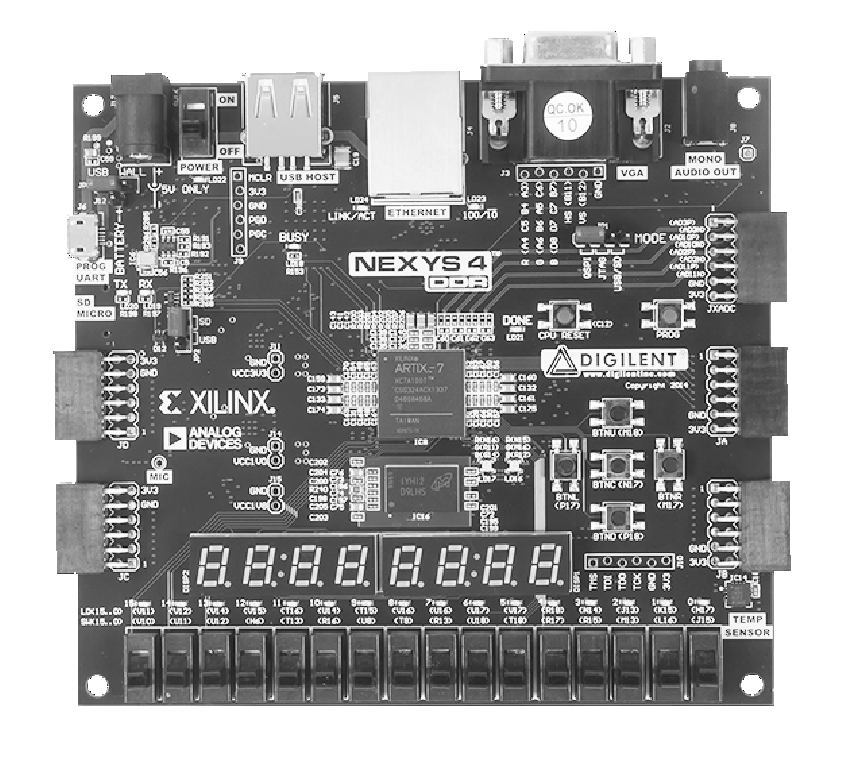
\includegraphics[width=0.6\columnwidth]{FPGA_board.eps}
	\caption{FPGA Nexys 4 DDR 开发版}
	\label{fig_board}
\end{figure}
\subsection{实验内容}
在算法分析及系统架构设计章节,本文详细的论述了系统设计的细节并展示了其所具有的潜在优势,例如从功能的角度,本文的系统设计能满足应用场景对
性能的弹性需求,能在资源有限的设备上独立运行,能实现和环境的数据交互等。从硬件实现的角度,本文所设计的硬件加速器具有高度复用的模块,极大的降低了
硬件资源的消耗。针对以上优势,本章设计了以下实验内容进行证明:

1.系统运行效果的实验:根据任务的难易程度以及任务的输入输出特点,本文选取了不同的测试集进行系统功能的测试。测试集包括单输入单输出系统:
NARMA10,NARMA30和复杂二阶问题,多输入单输出系统:耶拿天气预报数据集,多输入多输出系统:两入两出非线性系统。系统在运行这些任务时需要测试的功能
包括更改简化网络的模型尺寸,状态采样以及原始网络模型的压缩等。系统功能的正常是系统设计的首要目标,也是系统功能优势的实际体现。

2.加速器性能实验:本文对循环神经网络前向传播过程设计了专用硬件架构以实现加速的目的,加速器性能的主要指标有资源消耗,数据吞吐率(速度)以及功耗。
本实验将对这些指标分别进行测量,并将其与硬件设计相联系,说明本文加速器设计的特点和优势。

\section{系统运行效果}
实验设定:系统运行不同的任务,在连续输入的过程中切换模型尺寸,并以该尺寸的简化网络模型进行前向传播。简化网络模型的权重参数的生成有两种方法:
基于状态采样的模型生成方法和基于预置投影矩阵的模型生成方法,这两种方法分别对应系统的两种应用环境:异常状态环境和普通环境。在普通环境下,
网络的实际状态与预存的状态空间偏离较小,通过增大投影空间的方法可以实现状态的“准确”近似;在异常状态环境下,由于特征空间是有限的,无法囊括
所有的状态,少量实际存在的状态将在压缩的过程中被合理的丢失,然而在系统实际运行过程中难免会遇到这种情况,因此系统需要和实际环境进行数据交换,
通过采样的方法生成网络的权重参数。

本实验测量两种压缩模型生成方法下的模型预测效果。连续输入的序列长度为1000个,在完成该段序列的预测后,系统将会切换简化网络的模型尺寸并进行下一段序列的预测。
本实验依次设定简化网络模型阶数为10,20,30,40,60,80。实际上,在硬件支持的简化模型最大尺寸以下,简化网络模型尺寸可以设定为任意整数值。
%说明压缩算法能在边缘设备实现,加速器可以运行不同尺寸的网络模型。

\subsection{复杂二阶问题}
复杂二阶问题建模了一个二阶动态系统,该系统的数据依赖呈现指数相关的关系,即输入序列中的关键信息会被指数放大,而无关特征则会被迅速遗忘。
其数学表达为
\begin{equation}
	y(t+1) = \frac{y(t)y(t-1)(y(t)+0.25)}{1+y^2(t)+y^2(t-1)} + u(t)
\end{equation}
其中\(u(t)\)是在区间\([0,0.5]\)上生成的均匀分布的随机数。
\begin{center}
\begin{table}
	\caption{在二阶问题上不同尺寸简化网络模型的预测精度}
	\renewcommand\arraystretch{1.2}
	\setlength{\tabcolsep}{12pt}
	\begin{tabular}{ccccccc}
	\toprule
		 							&	10		&	20		&	30		&	40		&	60		&	80		\\	\midrule
	Sample M.\(\times 10^{-4}\)	&	2.99	&	2.58	&	2.46	&	0.81	&	0.25	&	0.11	 \\	\hline
	PreStore M.\(\times 10^{-4}\)&	36.3	&	18.5	&	9.9		&	6.9		&	1.7		&	0.53	\\	
	\bottomrule
	\label{tab:second}
	\end{tabular}
\end{table}
\vspace{-3em}
\end{center}



系统在二阶问题任务上的运行效果如图~\ref{fig:second} 所示,可以看出不同尺寸的简化网络模型的预测值均能较好的还原系统的真实输出。这里系统的真实输出可以
用原始网络模型的预测值进行准确的代替,一方面是因为原始网络模型的输出和系统真实输出误差较小,另一方面是因为在实际情况下测量系统的真实输出一般具有
滞后性,并且可能存在测量成本大等无法获得真实数据等情况。图中左侧是基于采样方法生成的简化网络模型,由上至下,模型的阶数依次增加。其中10阶的简化网络模型
预测效果和系统真实输出存在明显的偏差,随着简化网络模型尺寸的增大,模型的预测逐渐贴合系统的真实输出。图中右侧为基于预置投影矩阵方法生成的简化网络模型,
图中显示,该方法生成的简化网络模型在不同的模型尺寸下均拥有较小的误差。这说明小尺寸网络模型依然能胜任二阶问题的模型预测,网络精度的调节可以在
小尺寸网络的基础上进行小幅度改变即可。

表~\ref{tab:second} 展示了两种模型生成方法下简化网络不同尺寸的预测精度,误差的数值随着模型尺寸的增加而降低,其中采样方法生成的简化网络误差
降低更加明显。这说明了状态空间中越大,状态信息越丰富,其所生成的投影空间和和真实的特征空间偏差越小。由于预置的投影矩阵的生成往往采样了
足够多的状态数据,因此即使在相同的模型尺寸下,通过预存投影矩阵的方法生成的模型预测精度高于现场采样生成模型的精度。但是这并不能说明采样
方法不是系统所需要的功能。相反,由于该方法不依赖于任何先验信息,可以和环境交互数据,这使得即使系统处在异常环境中,也具有较高的预测能力。
两种方法互为补充,共同实现系统高精度预测的功能。
\begin{figure}
	\centering
	\subfloat[]
	{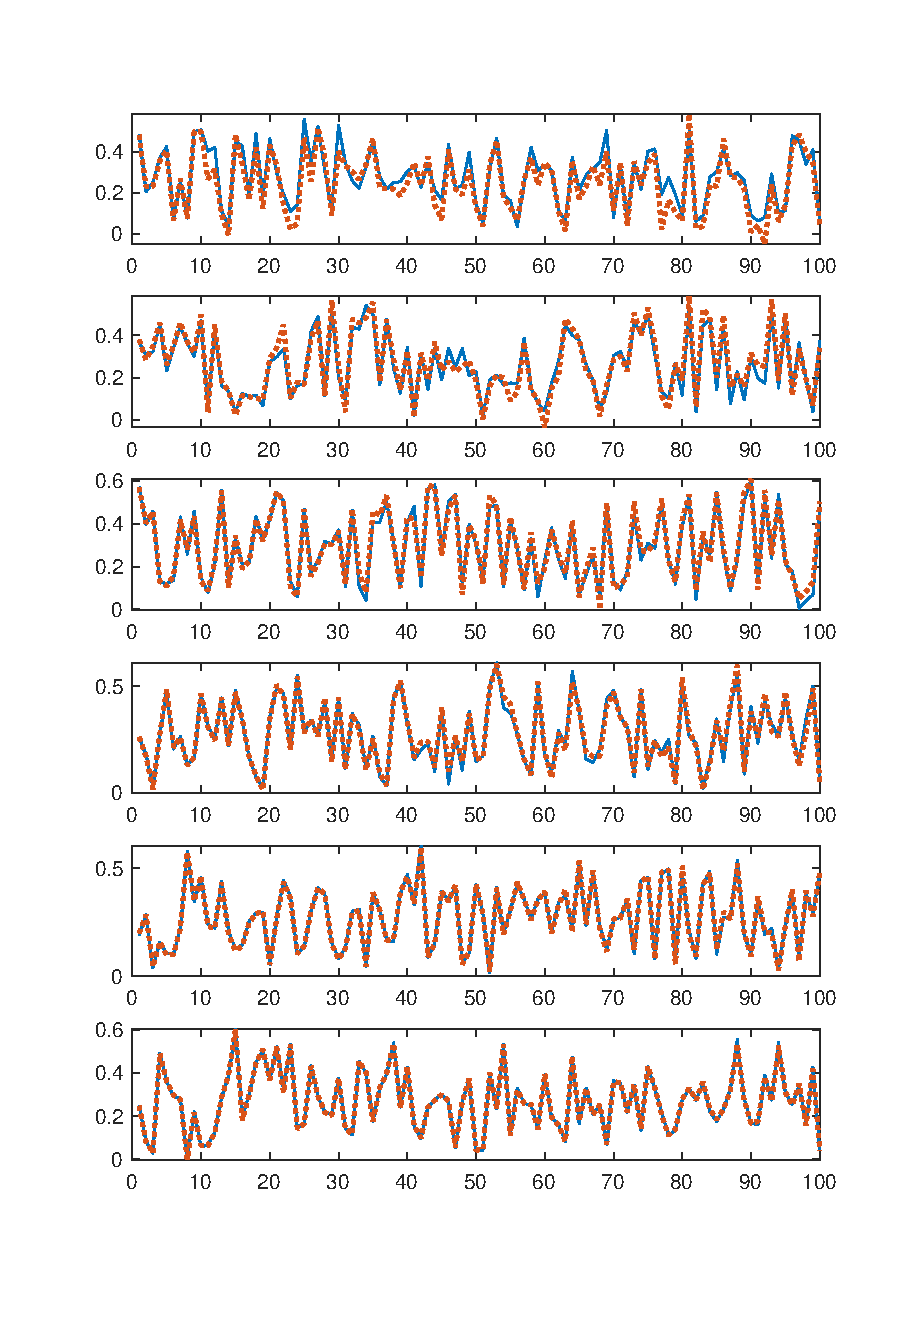
\includegraphics[width=0.5\columnwidth]{exp/fig_second_gen.eps}\label{fig:second_gen}}
	\subfloat[]
	{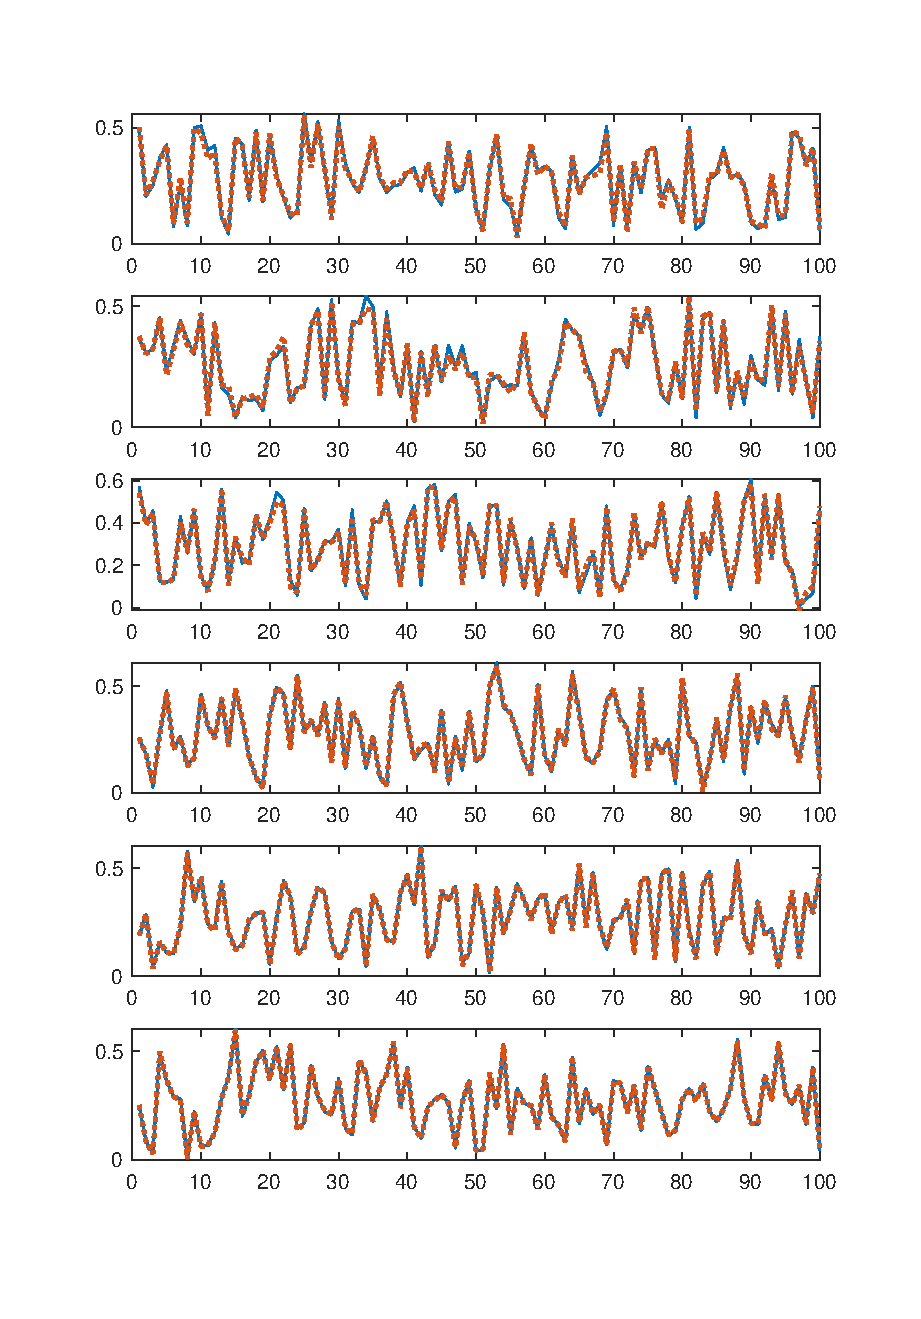
\includegraphics[width=0.5\columnwidth]{exp/fig_second_pre.eps}\label{fig:second_pre}}
	\caption{在复杂二阶问题上的系统运行效果,实线表示原始网络的预测值,点线表示简化网络的预测值。
		图a是使用采样方法的系统预测效果,图b是使用预存投影矩阵方法的系统预测效果。图a和图b自上而下的子图的简化网络阶数分别为10,20,30,40,60,80阶。}
	\label{fig:second}
\end{figure}


本文所设计的系统在二阶问题的任务的解决上,系统能够发现应用的实现难度较低进而主动降低简化网络模型的尺寸,并以较小的模型尺寸进行前向传播,
实现了高速的模型预测。相较于其他神经网络加速方法的一次性设计,本文的系统对应用的难易具有一定的感知能力。

\subsection{两个NARMA系统}

NARMA(Nonlinear Auto Regressive Moving Average)定义了具有长期依赖关系的动态系统,即很久以前的输入对系统当前的输出仍存在影响。循环神经
网络尽管能够学习这些长程依赖关系,但是依然存在一些难以解决的问题,例如对处理此类任务的循环神经网络进行压缩。压缩过程中损失的信息可能导致
网络失去长期记忆进而功能瘫痪。本文选取该应用进行系统运行效果测试,以验证系统在长期记忆的复杂任务中依然具有适用性。NARMA10系统的数学表达为
\begin{equation}
	y(t) = 0.3y(t-1) + 0.05y(t-1)\sum_{i=1}^{10}y(t-i) + 1.5u(t-9)u(t) + 0.1
\label{eq:narma10}
\end{equation}
NARMA30系统的数学表达为
\begin{equation}
	y(t) = 0.2y(t-1) + 0.04y(t-1)\sum_{i=1}^{30}y(t-i) + 1.5u(t-29)u(t) + 0.001
\label{eq:narma30}
\end{equation}
由式~\ref{eq:narma10} 和~\ref{eq:narma30} 可知,这两个系统的最大延迟时间步长分别为10和30。
\begin{figure}
	\centering
	\subfloat[]
	{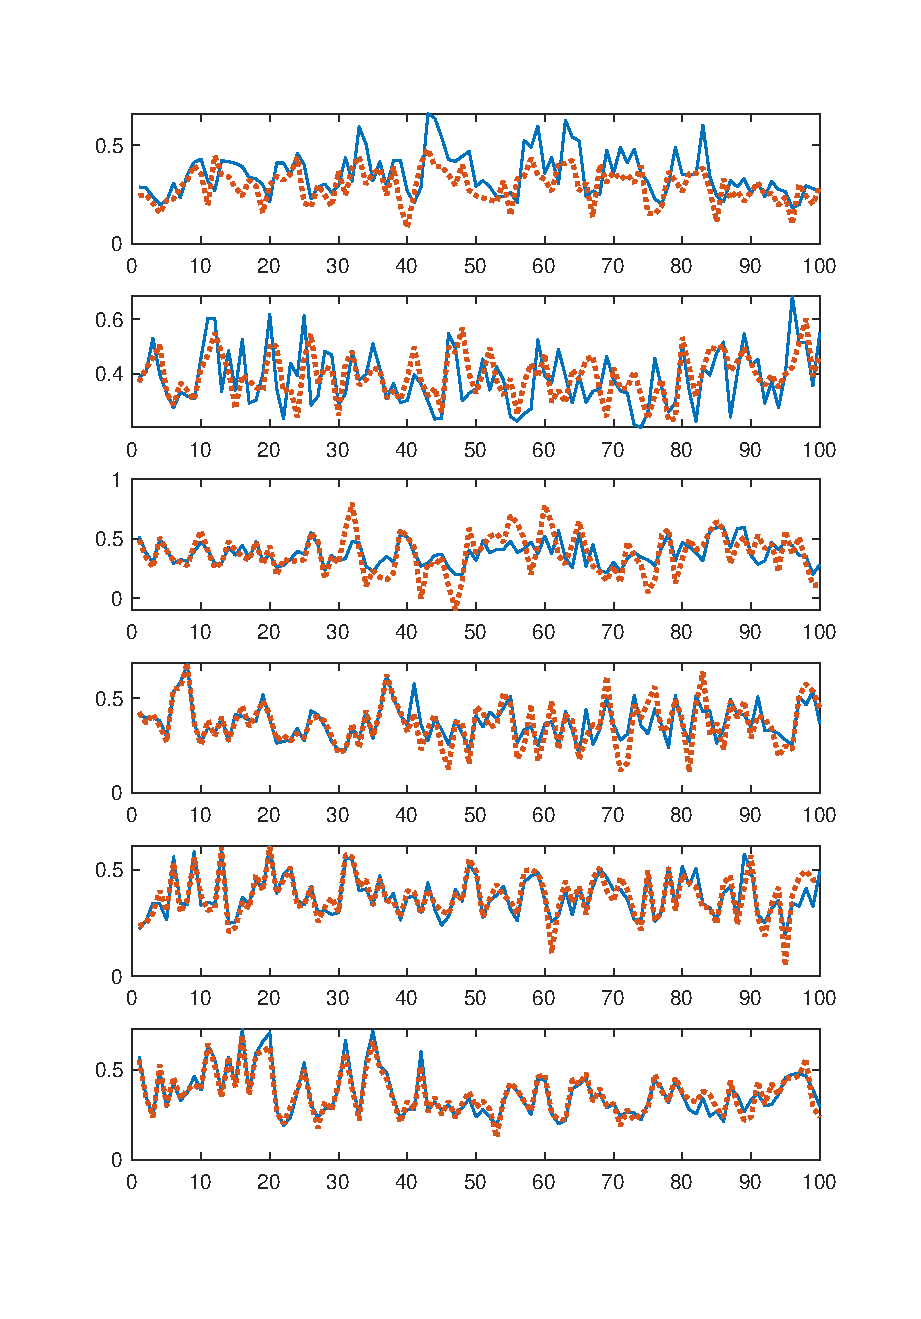
\includegraphics[width=0.5\columnwidth]{exp/fig_narma10_gen.eps}\label{fig:narma10_gen}}
	\subfloat[]
	{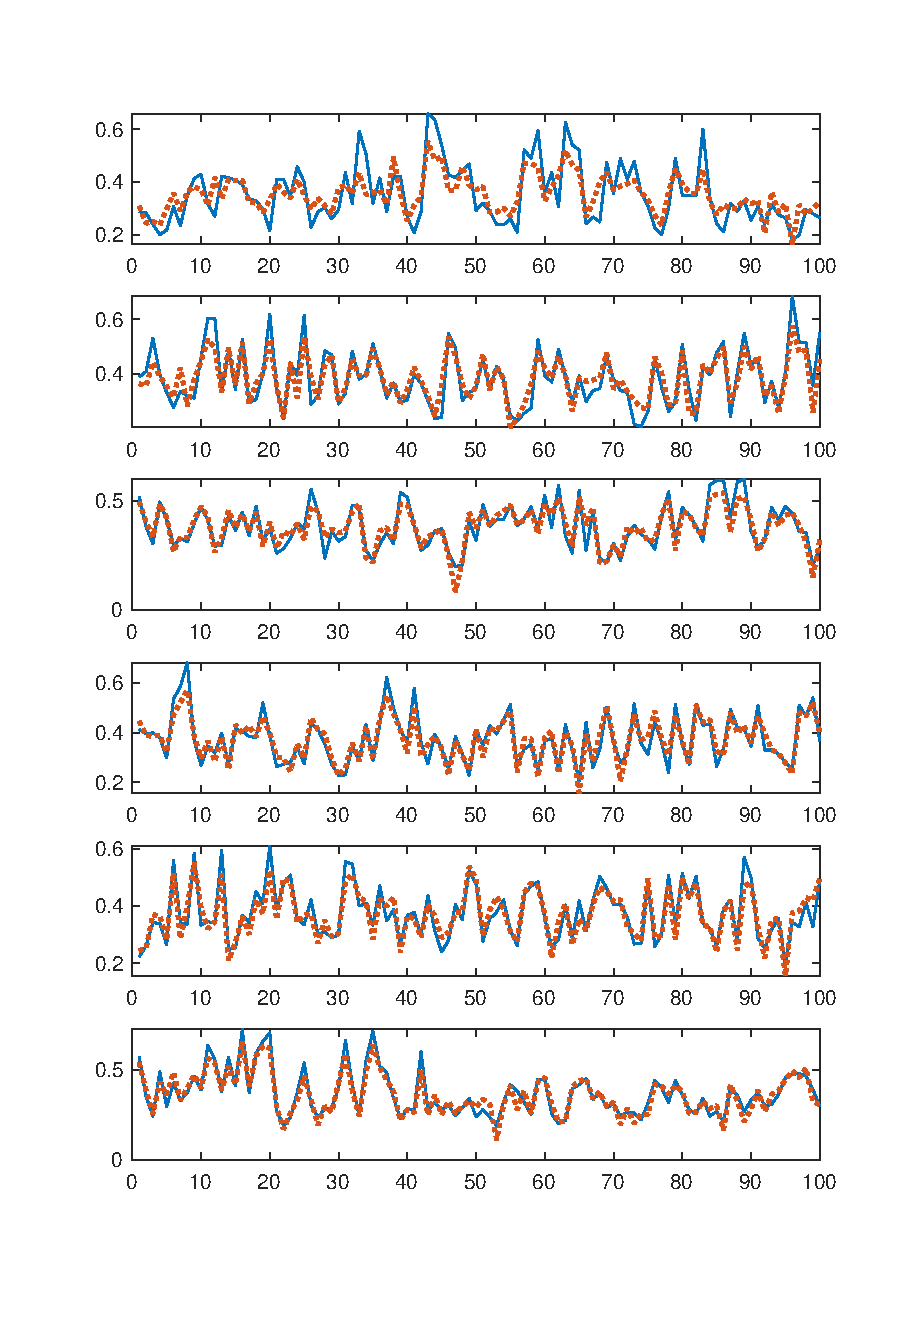
\includegraphics[width=0.5\columnwidth]{exp/fig_narma10_pre.eps}\label{fig:narma10_pre}}

	\caption{在NARMA10任务上的系统运行效果,实线表示原始网络的预测值,点线表示简化网络的预测值。
		图a是使用采样方法的系统预测效果,图b是使用预存投影矩阵方法的系统预测效果。图a和图b自上而下的子图的简化网络阶数分别为10,20,30,40,60,80阶。}
	\label{fig:narma10}
\end{figure}

\begin{center}
\begin{table}
	\caption{在NARMA10任务上不同尺寸简化网络模型的预测精度}
	\renewcommand\arraystretch{1.2}
	\setlength{\tabcolsep}{12pt}
	\begin{tabular}{ccccccc}
	\toprule
		 							&	10		&	20		&	30		&	40		&	60		&	80		\\	\midrule
	Sample M.\(\times 10^{-3}\)		&	4.2		&	1.7		&	1.6		&	1.5		&	1.3		&	1.2	 \\	\hline
	PreStore M.\(\times 10^{-3}\)	&	13.4	&	4.3		&	9.4		&	5.1		&	2.6		&	1.6	\\	
	\bottomrule
	\label{tab:narma10}
	\end{tabular}
\end{table}
\vspace{-3em}
\end{center}


图~\ref{fig:narma10} 所示为系统在NARMA10任务上的运行效果。由于任务的复杂度变高,小尺寸的简化网络模型在该任务上预测误差较大,其只能捕捉任务的变化趋势,
而对任务的具体细节则无法准确预测。当模型尺寸在40阶及其以上时,两种方法所生成的简化网络模型均能较好的预测任务的真实输出。对比两种模型生成方法下的网络
预测效果,当网络尺寸较大时,两种方法能获得相似的预测精度,在某段序列的预测上,采样方法甚至能获得更高的精度;当网络尺寸较小时,由于采样的的状态数量少,投影空间
包含的特征信息少,因此预测效果较基于预置投影矩阵的方法误差更大。
\begin{figure}[htb]
	\centering
	\subfloat[]
	{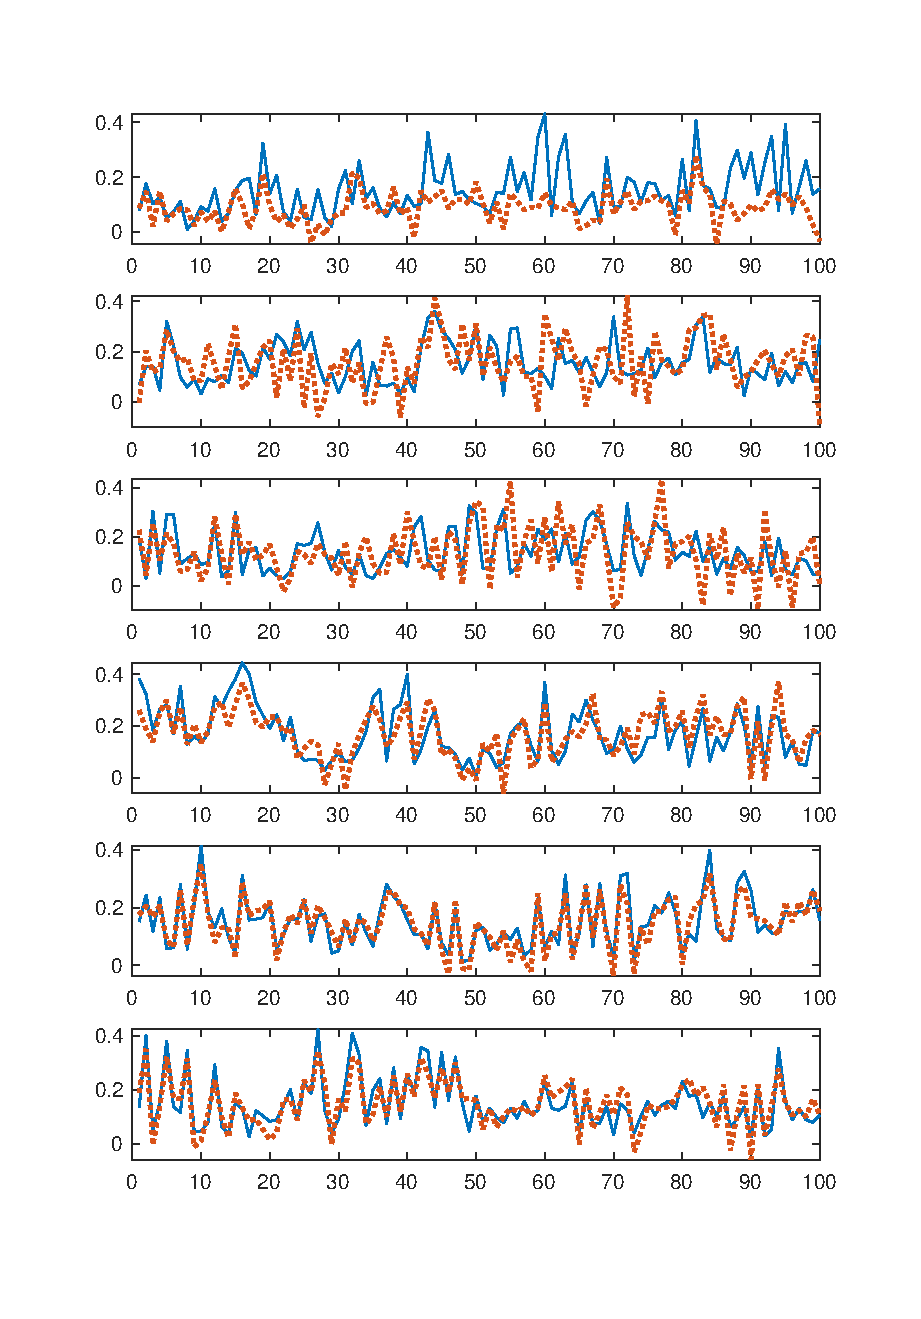
\includegraphics[width=0.5\columnwidth]{exp/fig_narma30_gen.eps}\label{fig:narma30_gen}}
	\subfloat[]
	{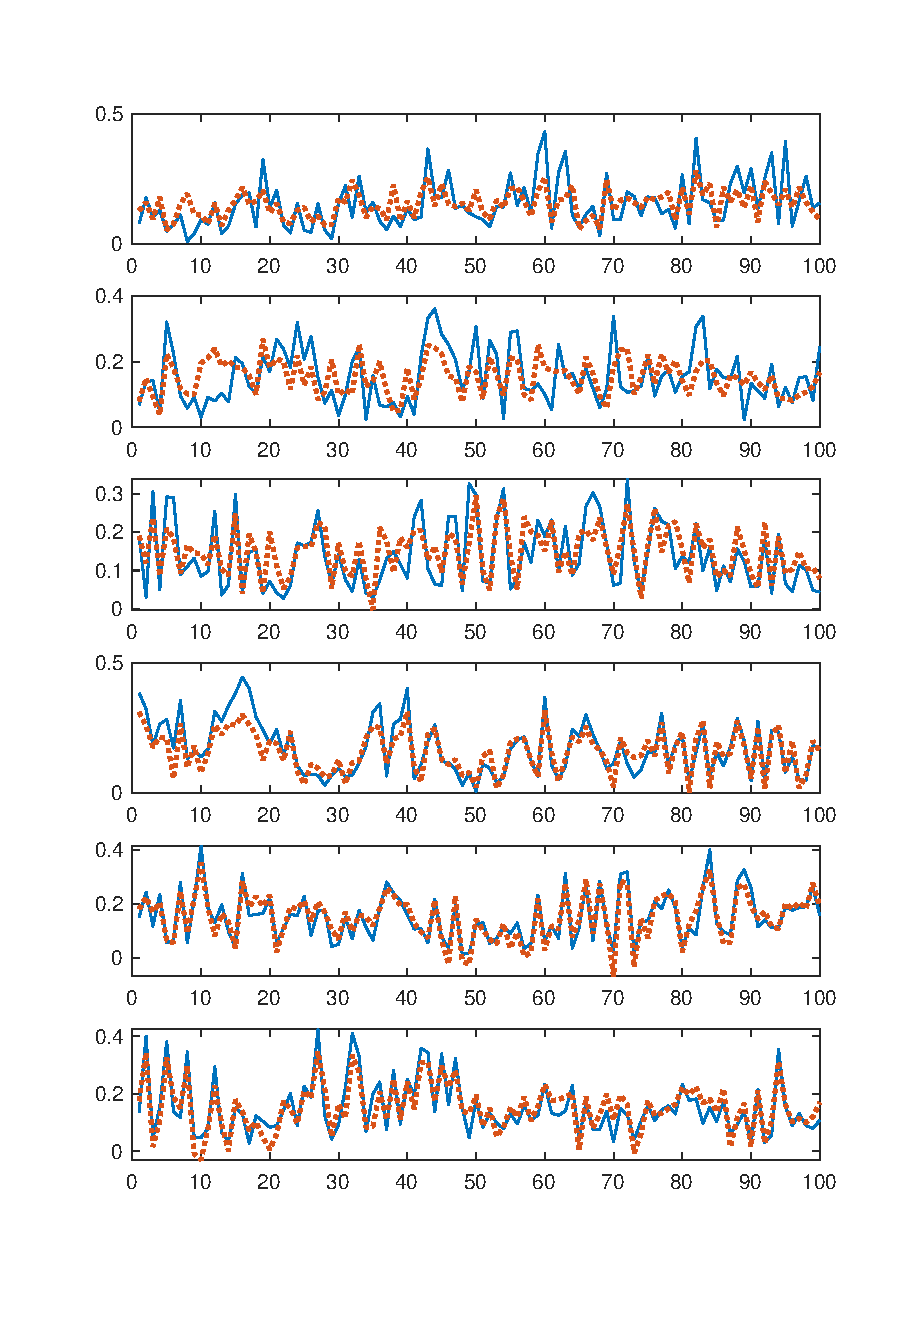
\includegraphics[width=0.5\columnwidth]{exp/fig_narma30_pre.eps}\label{fig:narma30_pre}}
	\caption{在NARMA30任务上的系统运行效果,实线表示原始网络的预测值,点线表示简化网络的预测值。
		图a是使用采样方法的系统预测效果,图b是使用预存投影矩阵方法的系统预测效果。图a和图b自上而下的子图的简化网络阶数分别为10,20,30,40,60,80阶。}
	\label{fig:narma30}
\end{figure}
\begin{center}
\begin{table}
	\caption{在NARMA30任务上不同尺寸简化网络模型的预测精度}
	\renewcommand\arraystretch{1.2}
	\setlength{\tabcolsep}{12pt}
	\begin{tabular}{ccccccc}
	\toprule
		 							&	10		&	20		&	30		&	40		&	60		&	80		\\	\midrule
	Sample M.\(\times 10^{-3}\)		&	5.1		&	5.0		&	3.3		&	1.7		&	1.4		&	1.3	 \\	\hline
	PreStore M.\(\times 10^{-3}\)	&	10.1	&	26.6		&	17.7		&	5.3		&	2.6		&	2.4	\\	
	\bottomrule
	\label{tab:narma30}
	\end{tabular}
\end{table}
\vspace{-4em}
\end{center}


图~\ref{fig:narma30} 所示为系统在NARMA30上的运行效果,相比于NARMA10,任务更加复杂。因此当简化网络模型的尺寸在60阶及其以上时,系统的预测才能较好的贴合
任务的真实输出,而在小网络尺寸例如10阶的简化网络模型,系统甚至难以预测任务的变化趋势。

系统在两个NARMA任务上的预测精分别如~\ref{tab:narma10} 和~\ref{tab:narma30} 所示。随着简化网络模型尺寸的增大,系统的误差也在不断降低。其中基于预存投影矩阵的简化网络
生成方法的精度变化不明显,而采样方法的误差会大幅降低。在以上两个基本规律下,存在个别反常现象,例如在NARMA30任务上10阶的模型的预测精度较低。这是因为系统对
环境数据进行采样时,样本点之间的相关性较弱,这使得样本集的信息量增加,对系统真实行为的相似度越高。这也说明,样本点对系统精度存在较大的影响,而现场采样
正是对预存采样信息的有效补充,因此采样方法也是保证系统独立性的重要环节。

本文所设计的系统在对复杂任务的处理上,不同模型尺寸的预测效果表现出较大的差异,系统可利用该特性实现系统唤醒以及精细化处理等功能。当任务在实际环境中
的重要程度不高时,系统运行小尺寸的网络模型,仅保留对任务的基本处理能力;当环境需要依赖该任务的处理结果时,系统可以切换到较高的模型尺寸进行精细化的处理。

\subsection{两输入两输出非线性系统}
从动态系统的输入输出数量的角度,前面的实验都是在单输入单输出任务上进行测试。为验证本文所设计的系统在多输入多输出的任务上具有适用性,本小节
的实验选取了两输入两输出非线性系统作为测试任务,其数学表达为
\begin{equation}
	\begin{split}
		&x_1(t) = 0.5x_1^{2/3}(t-1) + 0.3x_2(t-1)x_3(t-1) + 0.2u_1(t)	\\
		&x_2(t) = 0.5x_2^{2/3}(t-1) + 0.3x_2(t-1)x_1(t-1) + 0.2u_1(t)	\\
		&x_3(t) = 0.5x_3^{2/3}(t-1) + 0.3x_1(t-1)x_3(t-1) + 0.2u_2(t)	\\
		&y_1(t) = 0.7(x_1(t) + x_2(t))									\\
		&y_2(t) = 1.5x_1^{2}(t)	
	\end{split}
\label{eq:2In2Out}
\end{equation}
式中\(x_1,x_2,x_3\)是动态系统的三个状态,\(u_1,u_2\)是两个输入,输入的取值是\([0,0.5]\)区间内的均匀分布随机数,\(y_1,y_2\)是两个输出。

系统在两输入两输出任务上的运行效果如图~\ref{fig:2In2Out} 所示。其中误差最明显的系统运行效果来自于使用采样方法生成的10阶简化网络模型,
系统的预测与任务的真实输出存在一个固定的偏差值,这主要是由于采样的状态信息不够丰富。为了提高压缩过程的实现速度,本文设置采样的状态数量
和需要生成的简化网络模型阶数相同。随着简化网络模型尺寸的增加,采样方法生成的简化网络的模型将会消除这种偏差,并能以较高的精度还原任务的真实
输出。这说明采样方法存在缺陷,该方法生成的模型只能在采样的时间点附近拥有较高的精度,而在远离采样点的时刻则会精度较低。因此采样方法适用
于异常状态环境,系统能使用此方法在一段时间内获得精度方面的显著增益。但普通环境由于需要长时有效,因此一般选用预存投影矩阵的方法
生成简化网络模型。

表~\ref{tab:2In2Out} 展示了系统在两输入两输出任务上的模型预测精度。除过使用采样方法生成10阶简化网络模型的预测误差较大以外,其他的网络模型
均能实现较高的精度。实际上,系统在该任务上的最差的预测仍然能捕获任务的动态变化特性。

\begin{figure}
	\centering
	\subfloat[]
	{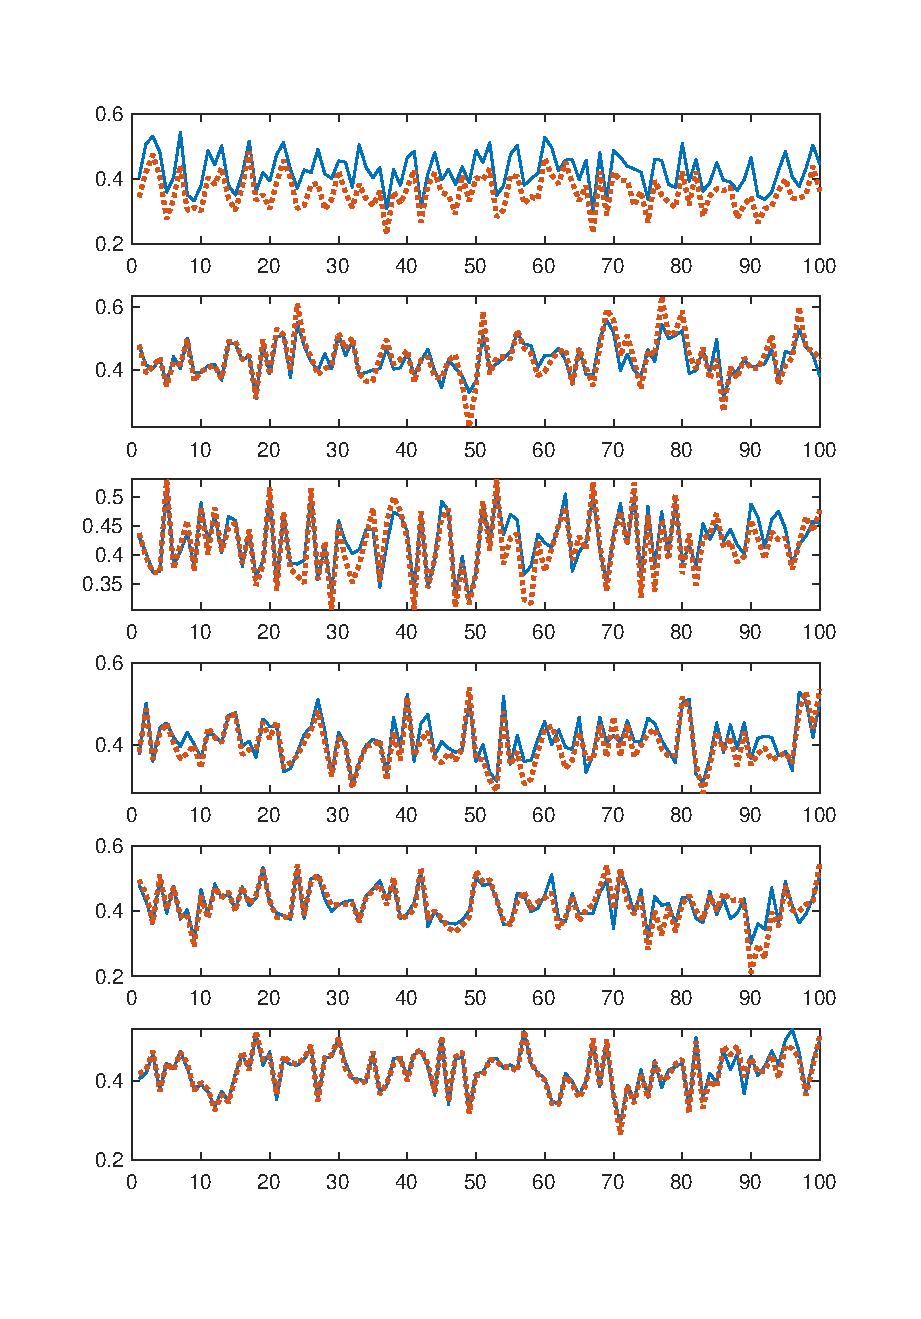
\includegraphics[width=0.5\columnwidth]{exp/fig_2In2Out_gen.eps}\label{fig:2In2Out_gen}}
	\subfloat[]
	{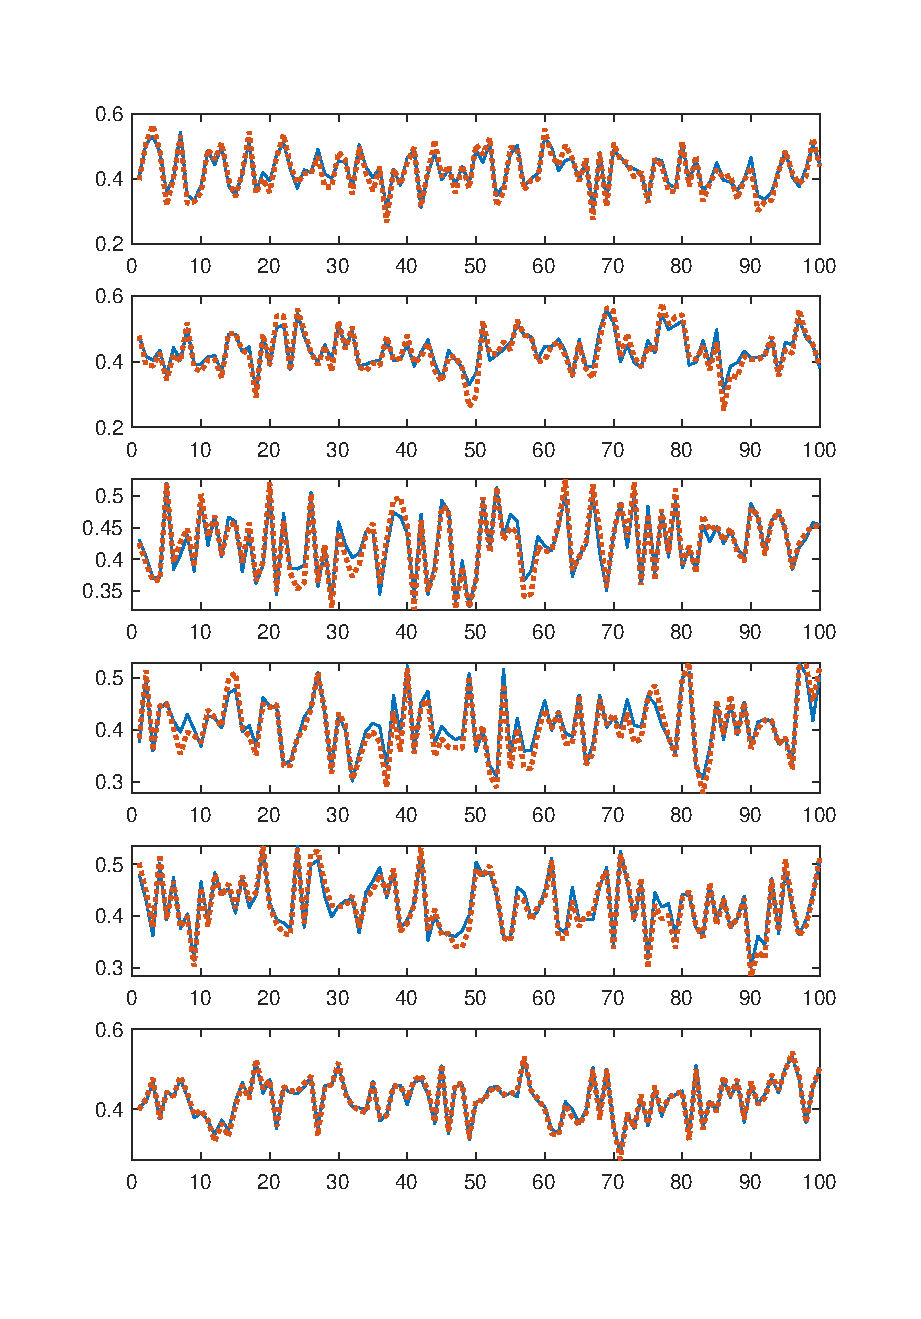
\includegraphics[width=0.5\columnwidth]{exp/fig_2In2Out_pre.eps}\label{fig:2In2Out_pre}}
	\caption{在两输入两输出非线性问题上的系统运行效果,实线表示原始网络的预测值,点线表示简化网络的预测值。
		图a是使用采样方法的系统预测效果,图b是使用预存投影矩阵方法的系统预测效果。图a和图b自上而下的子图的简化网络阶数分别为10,20,30,40,60,80阶。}
	\label{fig:2In2Out}
\end{figure}
\begin{center}
\begin{table}
	\caption{在两输入两输出非线性问题上简化网络不同模型尺寸的预测精度}
	\renewcommand\arraystretch{1.2}
	\setlength{\tabcolsep}{12pt}
	\begin{tabular}{ccccccc}
	\toprule
		 									&	10		&	20		&	30		&	40		&	60		&	80		\\	\midrule
	Sample M.~(\(\times 10^{-4}\))			&	4.8		&	3.1		&	2.2		&	2.1		&	1.6		&	0.6	 \\	\hline
	PreStore M.~(\(\times 10^{-4}\))	&	67.4	&	6.7		&	8.1		&	7.2		&	6.5		&	4.7	\\	
	\bottomrule
	\label{tab:2In2Out}
	\end{tabular}
\end{table}
\vspace{-3em}
\end{center}



本文所设计的系统能够胜任多输入多输出任务,并且配备了完善的解决方案以适应不同的运行环境。当系统运行在普通环境时,简化网络模型的生成一般
选用预存投影矩阵的方法;当系统运行在异常状态环境时,通过采样的方法获取异常状态信息,系统能在异常环境中获得较高的精度增益。%改进空间:将异常状态合并到投影矩阵中。
\\

经过以上不同类型任务的测试,本文所设计的系统均表现出良好的兼容性。首先系统的功能基本正常, 系统在运行过程中能切换简化网络模型的尺寸并以设定的尺寸进行
前向传播,网络的权重参数可以通过状态采样方法和预存投影矩阵的方法生成。在以上前向传播和网络压缩功能的相互配合下,系统表现出更高级的功能特性。
系统对任务,环境和用户需求存在一定的感知能力并能做出相应调整,例如根据任务的难易程度和精度要求,系统能动态调节简化网络的模型尺寸;当系统运行在
异常状态环境下,系统使用状态采样的方法以获取一段时间内的较高精度增益。此外,系统还表现出独立性与功能的完整性,系统基于FPGA平台实现,不需要额外的算力
和数据支持。综上所述,本文的系统满足设计目标,并表现出符合预期的优势。
%采样方法 样本覆盖的位置精度高

%在该类应用中的优势

%最后对系统运行效果进行总结


\section{加速器性能实验}

加速器负责实现前向传播过程,而该过程是系统最主要的功能,因此测量加速器的性能是必要的,其在一定程度上也能反映出系统的整体性能。本小节将从
速度,资源消耗以及功耗等方面对性能进行分析与测量。由于加速器的性能仅决定于加速器的硬件设计与实现,而与具体的任务关联度较小,所以
本实验的吞吐率(速度)和功耗数据都是系统运行NARMA10任务时采集的。
\subsection{吞吐率}
吞吐率是最直观的衡量系统运行速度和延迟的综合性指标,其含义是单位时间处理的系统输入的数量。影响吞吐率的因素主要包括系统频率,运算量,访存延迟等,
是系统各个要素综合作用的结果。本文所设计的加速器结构能够运行不同网络模型:包括原始网络模型和简化网络模型,能够更改网络模型的尺寸:本文主要是指
简化网络的尺寸。以上各种系统运行模式存在不同的计算量和存储量,因此也存在吞吐率的差异。差异化的吞吐率即代表着系统推理的速度可以调节,这能满足用户
和环境对速度的弹性化需求,也是本文系统设计的主要特点之一。

本实验分别测量不同网络结构和不同模型尺寸条件下任务的完成时间作为计算吞吐率的依据,任务的序列长度为10000个,加速器的运行频率是100MHz,时间的计量
采用任务进行标记和串口输出的方式实现。实际上,吞吐率和任务的完成时间呈倒数关系,两者表示的是同一事物,本文更形象且方便的描述其为速度。

表~\ref{tab:time} 所示为加速器以不同尺寸的网络模型处理10000个序列输入消耗的总时间。其中500表示原始网络,其余阶数表示简化网络的尺寸。
从表中可以看出,在处理相同的任务量的条件下,原始网络消耗的时间远大于简化网络,其所产生的高昂时间成本严重阻碍了网络在实际环境中应用。
相比于原始网络,使用模型压缩技术生成的简化网络则拥有较低的时间延迟,表中所示的最小速度提升都能达到29倍,随着简化网络尺寸的减小,速度最大提升幅度
可达265倍。仅从速度的角度考虑,系统应当运行延迟更小简化网络模型。理论上,在简化网络模型中,不同尺寸的模型之间的速度提升应当呈现一定的相关性,具体可见公式~\ref{eq:computeComplexity},
但是由于硬件的实现需要考虑并行与串行,存储的突发传输等因素,实际的加速比例较理论值存在差异。这说明神经网络的实际加速能力不仅取决于算法的时间复杂度,即本文的模型尺寸,
还受到硬件实现的约束。
\begin{center}
\begin{table}
	\caption{不同尺寸的网络模型完成10000个序列输入消耗的时间}
	\renewcommand\arraystretch{1.2}
	\setlength{\tabcolsep}{10pt}
	\begin{tabular}{cccccccc}
	\toprule
		 		&		500		&	10		&	20		&	30		&	40		&	60		&	80		\\	\midrule
	Time(ms)	&		486121	&	1833	&	2729	&	4093	&	5907	&	10457	&	17031 \\	\hline
	Speed up	&		\#		&	265		&	178		&	119		&	82		&	47		&	29 \\
	\bottomrule
	\label{tab:time}
	\end{tabular}
\end{table}
\vspace{-3em}
\end{center}

%Time(ms)	&		486121	&	1833		&	2729	&	4093	&	5907	&	10457	&	17031 \\	\hline

\begin{center}
\begin{table}
	\caption{不同尺寸的网络模型浮点计算能力}
	\renewcommand\arraystretch{1.2}
	%\setlength{\tabcolsep}{8pt}
	\begin{tabular}{cccccccc}
	\toprule
		 				&		500		&	10		&	20		&	30		&	40		&	60		&	80		\\	\midrule
		Perf~(FLOPS)		&		534846	&	1745772	&	4543788	&	6743220	&	8261385	&	10442766&	11367506	\\	\hline
		Perf.imprv		&		\#		&	3.26	&	8.5		&	12.6	&	15.5	&	19.5	&	21.3	\\
	\bottomrule
	\label{tab:flops}
	\end{tabular}
\end{table}
\vspace{-3em}
\end{center}


根据表~\ref{tab:accuracy}中的模型参数量和表~\ref{tab:time}的运行时间,不难获得不同尺寸模型的浮点运算能力,如表~\ref{tab:flops}所示。
相比于原始网络模型,在浮点计算能力方面,简化网络拥有更大的优势,并且随着简化网络尺寸的增加,优势也更加明显。尽管浮点计算能力随着简化网络
模型的尺寸增大而提升,但是提升的幅度却逐渐变小。造成这一现象的原因是加速器的设计采用了流水线技术,随着模型尺寸的增加,流水线停顿所占的时间比例降低,
有效的数据处理周期数增加,因此加速器的浮点运算性能提升;另一方面,由于模型尺寸增大,加速器需要搬运的数据量也增加,数据的搬运包括从片外存储移动到
片上存储和在片上不同存储单元之间交换数据,数据移动会产生比较大的延迟,这会降低加速器的浮点性能。以上两点因素共同影响着加速器的浮点运算能力。

\subsection{运行功耗}

\begin{figure}
	\centering
	\includegraphics[width=0.4\columnwidth]{exp/fig_power.eps}
	\caption{使用功率计实测FPGA的运行功耗}
	\label{fig:power}
\end{figure}


\begin{center}
\begin{table}
\caption{简化网络和原始网络的运行功耗}
\renewcommand\arraystretch{1.3} 
\setlength{\tabcolsep}{12pt}{
\begin{tabular}{|c|c|c|c|}
\hline
						&	\multicolumn{2}{c|}{FPGA}	&	CPU		\\	\hline
						& Original ESN	&	Reduced ESN	&	ESN		\\	\hline
	Total Power~(W)		&	2.9			&	2.7			&	33.4	\\	\hline
	Dyanmic Power~(W)	&	1.7			&	1.5			&	23.1	\\	
\hline
\end{tabular}
}
\label{tab:power}
\end{table}
\end{center}
\vspace{-3em}


FPGA功耗包括静态功耗和动态功耗,其中静态功耗由泄漏电流引起,可通过测量系统在休眠状态下测量的功耗来获得;动态功耗由翻转功耗和短路功耗组成,
可通过测量系统在运行任务时的功耗来获取。本实验使用上述测量方法分别测量了系统的静态功耗和运行总功耗,并计算出静态功耗。

本实验测量了两种系统功能的运行功耗,分别是原始网络的运行功耗和简化网络的运行功耗,图~\ref{fig:power} 展示了本实验具体的测量方法。本实验
使用功率计实测系统的运行功耗,而不采用Xilinx提供的功率分析工具进行估算,其原因在于本文系统的两种网络类型存在较大的结构差异,一些电路
部件在原始网络的运行过程中会被频繁的使用,但是简化网络却使用频次较少,这种利用率的差异会导致系统实际运行功率也存在区别。Xilinx的功率分析
工具无法获取不同任务的利用率,只能估算的系统整体功耗。因此,本实验采用实测的方法。

简化网络和原始网络的运行功耗如表~\ref{tab:power}所示,系统运行原始网络的总功耗为2.9~W,运行简化网络的总功耗为2.7~W,系统的静态功耗为1.2~W。
静态功耗甚至和动态功耗相当,这说明系统在运行网络的前向传播任务时,系统中还存在其他的处于休眠状态的功能部件,实际上也正如此,例如CPU模块,AXI总线
模块等都处在极低的利用率状态。相比于原始网络,简化网络尽管结构更加更加复杂,但是其模型参数量更少,数据移动的次数更少,所以其运行功耗更低。
总体上,系统执行主要任务时最高功耗仅为2.9~W,可以适用于多数边缘应用场景,满足了本文对系统使用场景的设想。

\subsection{资源消耗}
FPGA拥有种类丰富的片上资源,包括LUT,BRAM,FF以及DSP。基于以上资源,开发人员可以构建定制化的硬件结构以实现算法加速的目的。但是FPGA的片上
资源也是有限的,在进行硬件架构设计时需要充分考虑资源的并行性和复用性。本文的设计充分考虑了资源消耗的因素,采用了神经网络结构层面的模块复用方法,
并对资源消耗大的功能组件进行了优化,最终以合理的资源消耗实现了系统的设计。


\begin{tabular}{ccccccc}
\toprule
	 &			&	LUT		&	LUTRAM	&	FF		&	BRAM	&	DSP	\\	\hline
 	 &	Avili.	&	63400	&	19000	&	126800	&	270		&	240 \\	\hline
\multirow{2}{*}{Accelerator}&	Used	&	21531	&	921	&	41048	&	29	&	66\\
							&	Utili.	&	33.96\%	&	4.85\%	&	32.37\%	&	10.74\%	&	27.59\%	\\
					\hline	
\multirow{2}{*}{SOC}		&	Used	&	45322	&	5410	&	66090	&	33	&	68\\
							&	Utili.	&	71.49\%	&	28.47\%	&	52.12\%	&	12.22\%	&	28.33\%	\\

\bottomrule
\end{tabular}



\begin{center}
\begin{table}
\caption{简化网络和加速器整体的资源消耗}
\renewcommand\arraystretch{1.2} 
\setlength{\tabcolsep}{8pt}{
	\begin{tabular}{cccccc}
	\toprule
		Resource	&		LUT		&	LUTRAM	&	FF		&	BRAM	&	DSP	\\	\hline
		Reduced ESN	&		17083	&	790		&	34611	&	22		&	65	\\
		Accelerator &		20610	&	921		&	41048	&	29		&	66	\\	
	\bottomrule
\end{tabular}
}
\label{tab:resourceESN}
\end{table}
\vspace{-3em}
\end{center}


表~\ref{tab:resourceUsed} 所示为本文所设计系统和硬件加速器的资源消耗情况。在系统消耗的资源中,加速器消耗占比最大的部分是DSP和BRAM,分别
代表计算资源和存储资源,这说明系统计算和存储的压力主要由加速器承担。实际上神经网络的前向传播是系统计算和存储需求最大的任务,而加速器
正是实现该任务的硬件平台,因此加速器资源消耗比例大也是正常现象。系统资源消耗中加速器占比较小的部分是LUT和FF,
这部分资源实现了MicroBlaze,Uart和AXI总线等功能部件,这些部件也是系统实现完整功能必不可少的部分,因此额外的资源消耗也是合理的。以上分析了
加速器和系统总体资源消耗的合理性,反映出本文在系统设计层面是经过合理规划的。

本文的加速器可以运行两种不同结构的网络模型,分别是原始网络和简化网络。考虑到两种网络存在相似的基本结构,本文采用模块复用的方法设计加速器的结构,
以达到节约资源并提高各硬件模块利用率的目的。表~\ref{tab:resourceESN} 所示为简化网络和加速器整体的资源消耗,其中简化网络在整个加速器的资源消耗中
占比可达80\%以上,DSP的比例甚至高达98\%。相比简化网络,加速器所增加的额外资源开销用以实现原始网络前向传播和状态采样等功能。从资源消耗的比例
和系统功能的重要程度来看,本文加速器的资源分配是合理的。
简化网络的前向传播是加速器实现的
主要功能,因此该部分硬件结构的设计遵循速度优先的原则。尽管简化网络中的各层神经元是均具有相似的结构,但该部分的硬件设计并未采用分时复用的方法,
而是设计独立的运算单元,这种资源换速度的策略也是常用的加速策略。对于系统的使用频次较低的功能,本文设计采用硬件结构共享的设计方法,例如原始网络和简化网络
存在大量相似的功能单元,因此原始网络共享了简化网络结构的一部分,主要体现在计算结构上,这也是DSP仅额外增加一个的原因。对于相似性较小的部分
则单独设计硬件结构,主要体现在存储单元上,原始网络所需存储的向量维度更大,因此系统所需的额外存储资源也较多,包括BRAM和LUTRAM。
额外消耗的FF主要用于加速器的控制单元,功能增加,控制逻辑也就更加复杂,控制单元消耗的资源也就越多。
\begin{center}
\begin{table}
\caption{分段近似方法的激活函数硬件资源消耗}
\renewcommand\arraystretch{1.2} 
\setlength{\tabcolsep}{16pt}{
	\begin{tabular}{ccccc}
	\toprule
		Resource	&		LUT		&	FF		&	BRAM	&	DSP	\\	\hline
		Tanh		&		6237	&	9512	&	6		&	43	\\
		Tanh Approx.&		1270	&	1137	&	0		&	5	\\	
	\bottomrule
\end{tabular}
}
\label{tab:resourceTanh}
\end{table}
\end{center}
\vspace{-3.5em}


表~\ref{tab:resourceTanh} 展示了分段近似激活函数的硬件资源消耗,其中Tanh是使用Xilinx提供的IP实现的,Tanh Approx是本文提出的分段近似激活函数
硬件实现方法。表中可以看出,近似方法实现的激活函数会大幅的降低各种硬件资源的消耗,其中DSP和FF资源消耗降幅可达九分之一,LUT的降幅为五分之一,
BRAM的开销甚至降低为0。这种资源降低是以牺牲激活函数的精度为代价而换取的,但只要精度损失不会影响系统功能的稳定和正常,这种交换就是值得的。
如果直接使用未优化的激活函数硬件模块,加速器的资源开销也将显著增加,相比于主要功能---简化网络前向传播结构,主要的资源增幅可达原来的三分之一,
甚至高于加速器其他功能所带来的额外资源消耗。以上分析说明本文对激活函数的优化是必需且有效的。


\section{本章小结}

本章基于FPGA硬件平台对本文所设计的循环神经网络加速系统进行测试,实验内容包括系统运行效果和硬件加速器的性能。在系统运行效果方面,本文基于FPGA
实现的系统能够完成网络模型压缩和网络的前向传播两大过程,系统的基本功能都经过了充分的验证,包括原始网络和简化网络的切换,调整简化网络模型尺寸,生成简化网络
模型权重参数等。为了证明本文所设计的系统能够适用于广泛的应用场景,实验测试了不同类型的任务和两种不同场景的简化网络模型生成方法,并且测量
出系统运行过程中的精度数据。在系统基本功能正常的前提下,加速器性能的实验分别从功耗,速度和资源消耗等方面对本文系统的特点进行详细说明。
系统的峰值总功耗为2.9W,简化网络的前向传播功能仅需要2.7W,系统的实现具有低功耗的特点,可以适用在多数边缘应用场景。在运行速度方面,系统
以不同尺寸的简化网络进行前向传播可以获得不同的加速能力,网络尺寸越小,加速能力越明显。通过将加速能力和模型预测精度这一组矛盾相结合,系统
可以满足用户对精度和速度的弹性需求。最后,在硬件资源消耗方面,本章分别从系统整体资源消耗,简化网络资源消耗以及激活函数的资源消耗等不同层面
详细展示了本文在资源优化方面的成果:系统采用了模块复用和结构共享的设计方式,在不超过简化网络资源开销的20\%的额外资源消耗下,硬件加速器
实现了系统其他低频使用的功能;分段近似的激活函数实现相较未优化节约了八成以上的资源开销。经过系统资源的优化设计后,系统实现所需要消耗的资源
大幅降低,能够迁移到其他资源有限的硬件平台运行。





%提高各个部件的利用率。
%由于FPGA系统的动态功耗和任务类型相关,更具体的,任务决定着芯片各个部件的利用率,当某个部件的被频繁使用时,那么该部件会产生较大的动态功率,
%如果某个部件的利用率较低,相应的,其功耗越接近静态功耗

%解释为什么要测量不同模型的功耗。

%\subsubsection{耶拿气候集}
%
%\begin{figure}
%	\centering
%	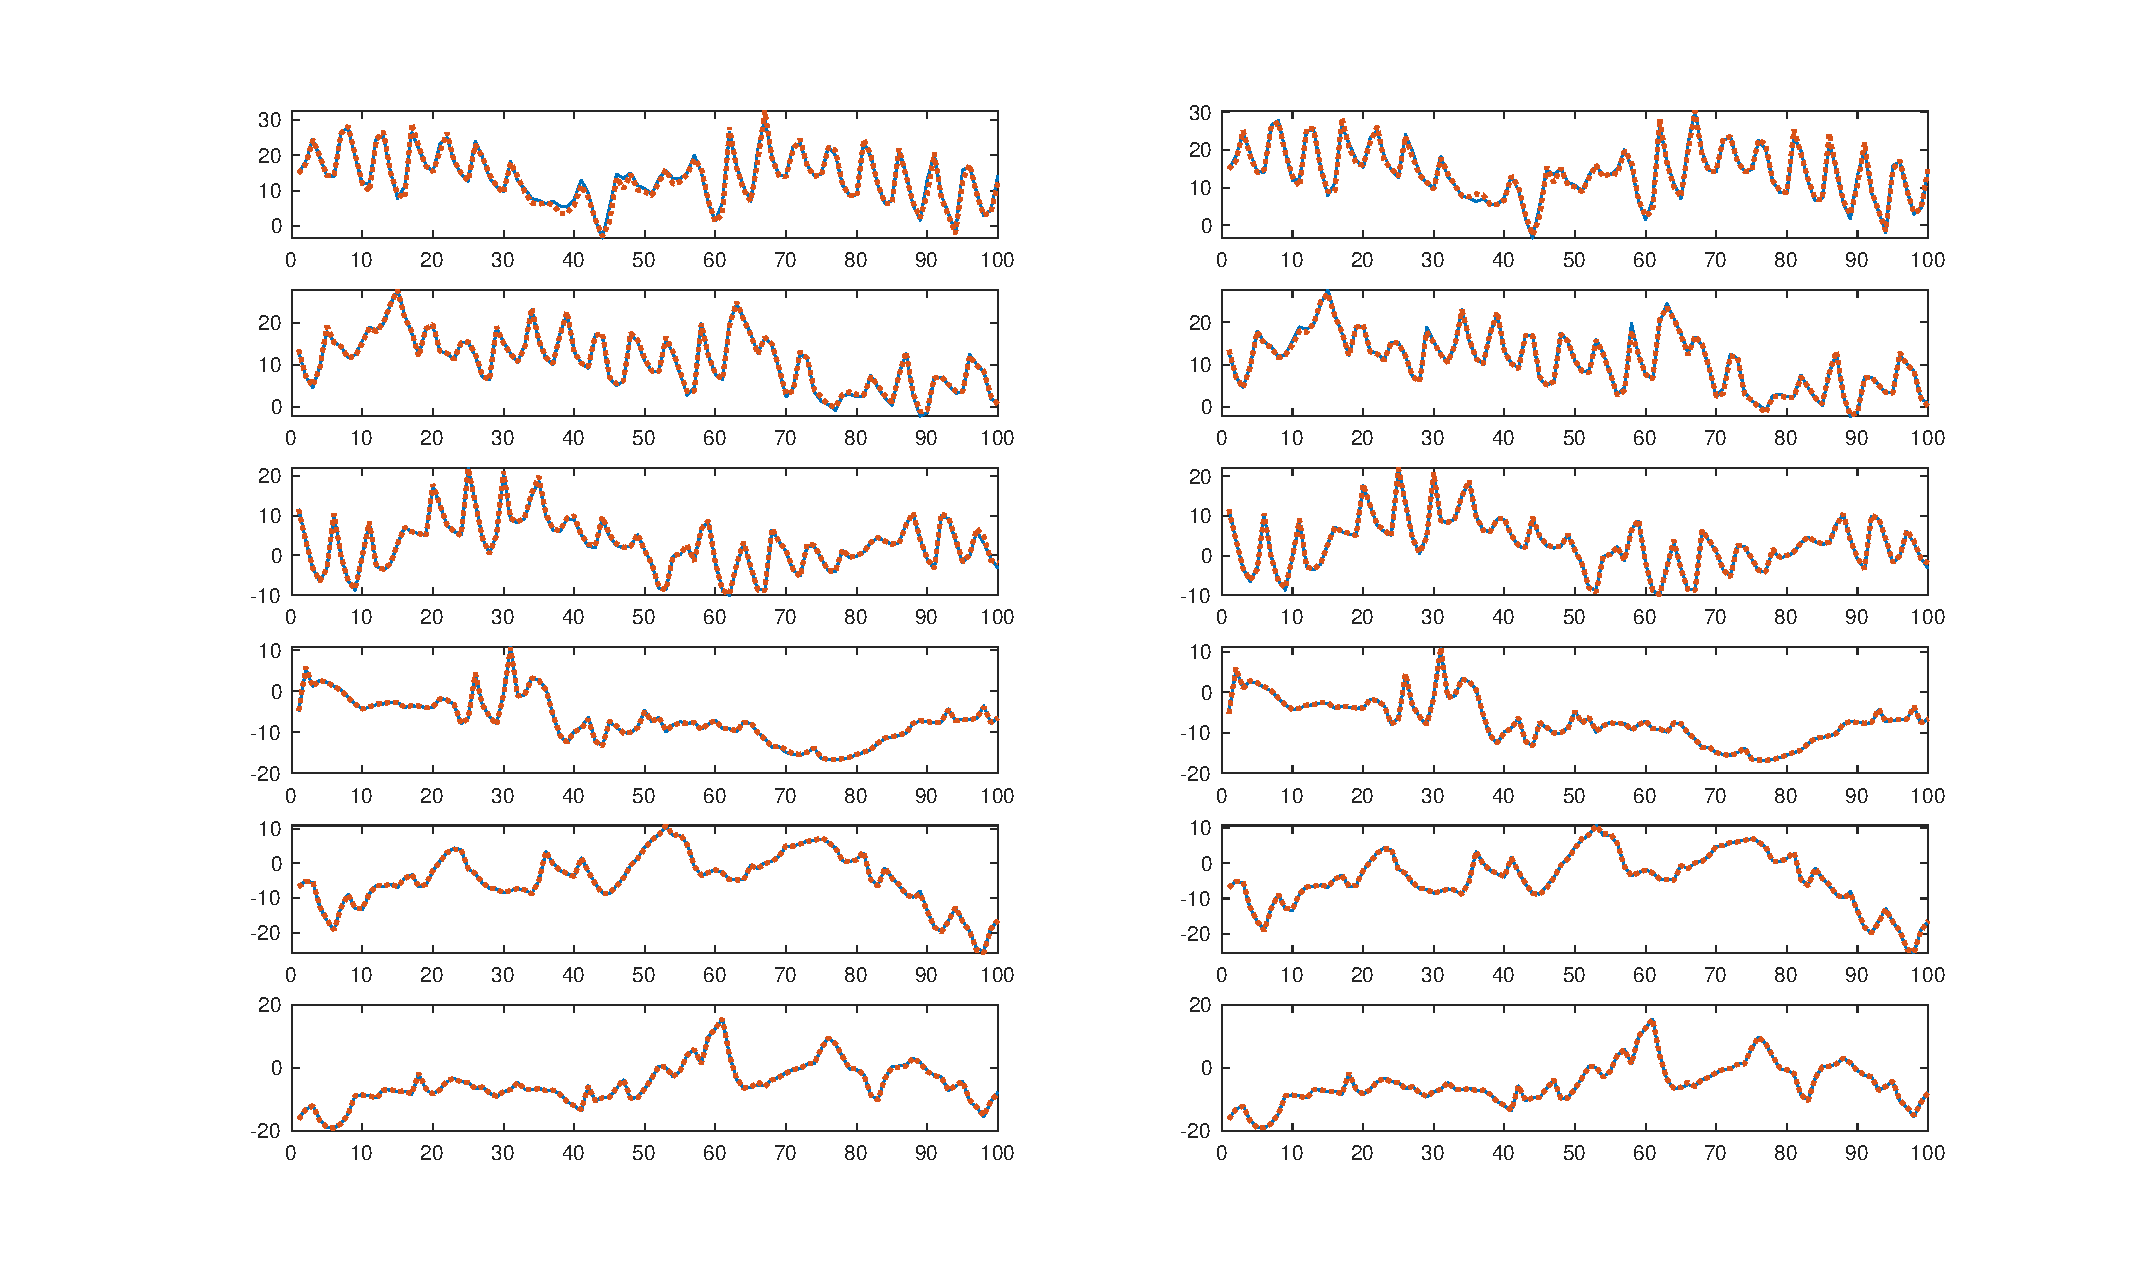
\includegraphics[width=1\columnwidth]{exp/fig_weather.eps}
%	\caption{在耶拿气候预测任务上的系统运行效果,图中左侧为使用采样方法生成简化网络,右侧为使用预存投影矩阵方法生成简化网络,图中自上至下表示的网络阶数分别
%	为10,20,30,40,60,80。实线表示原始网络的模型预测值,虚线表示简化网络的模型预测值。}
%	\label{fig:second}
%\end{figure}

\chapter{全文总结与展望}
至此,本文完成了循环神经网络加速系统的相关技术,系统流程,软硬件功能划分及实现,系统测试等全部工作的介绍。接下来,本章将在5.1节对本文的工作
进行总结并阐释本文工作的创新性,在5.2节将分析本文工作存在的问题,并对后续研究进行展望。
\section{全文总结}
在循环神经网络广泛应用的背景下,本文针对一类普遍存在的应用场景需求---动态调节速度和精度,设计并实现了循环神经加速系统。该系统将网络的压缩过程
和前向传播过程有机结合,实现了在系统运行过程中根据环境的需求生成特定尺寸的网络模型参数并进行前向传播的系统运行效果,达成了动态调节
循环神经网络预测精度和速度的目的。

首先,本文在分析压缩过程和网络前向传播过程特性的基础上进行了系统架构设计,从系统各功能模块的算法特征,系统时间占比以及实现成本等方面综合考虑
完成了系统的软硬件划分,其中压缩过程和系统控制交由软件实现,网络前向传播和状态采样则交由硬件实现。

其次,为了使系统在异常状态环境中仍能正常发挥预测功能,本文提出了基于预置投影矩阵的模型压缩流程和基于状态采样的模型压缩流程,分别用于普通环境
和异常状态环境。完善的应用环境设计使得系统具备了对环境的鲁棒性。

然后,为了降低网络前向传播过程的延迟,本文设计了针对循环神经网络前向传播过程的专用加速器。相比于传统加速器的一种硬件结构唯一对应
一种网络模型,本文所设计的加速器能够运行两种网络模型并且能调节网络的尺寸,具备一定的通用性。加速器的设计充分考虑了硬件资源的约束,采用了模块
共享和分时复用的技术。同时加速器也在不同的层面进行了并行化设计,依次为树形向量乘法,堆叠PE的计算单元,以及网络层的流水线并行。

接着,本文对硬件加速器中激活函数模块进行了优化。通过对比不同的激活函数硬件实现方式的资源消耗以及精度损失,本文最终采用了分段三次函数
近似的激活函数实现方法,在抽象出其基本运算单元后,本文设计了相应的激活函数硬件电路结构。
%为了系统高效的运转,本文依据各功能模块的算法特性,系统时间占比以及实现成本进行了软硬件划分

最后,本文基于FPGA实现了循环神经网络加速系统,并对系统功能的完整性以及加速器的性能进行了测试。实验结果表明本文所设计的系统具备动态调节精度和速度的
能力,能够胜任不同类型的任务。系统的资源消耗合理,在以不超过主要功能单元---简化网络结构资源消耗的20\%的条件下实现了其他的系统功能。系统的运行
功耗较低,可以应用于多数低功耗场景。系统具有较高的能量转换效率,在严格能量约束的条件下能高效的完成数据运算功能。

\section{后续工作展望}
本文仅从系统的有效性及可行性角度出发设计并实现了循环神经网络加速系统,距离系统真正的实际应用还存在一些改进空间。例如,本文系统仅对循环神经网络的前向传播
过程进行了硬件加速,而压缩过程则采用软件的实现方式,尽管这样的软硬件分工可以使得系统高效的运转,但是却存在压缩过程耗时较长等缺陷,这使得
系统的动态调节能力不具备实时性这一重要特征。针对实时性问题,可能存在的解决方案包括设计专门用于加速网络压缩过程的硬件加速器和使用高速异构硬件平台如高速CPU,GPU等。
此外,本文的研究是为动态调节网络精度速度场景而设计的,其系统设计流程和框架具备通用性,但是本文仅以循环神经网络作为研究对象,因为其具有低成本的
网络模型压缩算法,其他的模型压缩算法往往由于成本过高,现阶段无法实现,这就对开发低成本,无数据集的压缩算法提出了迫切的需求。

%\input{chapter/template}

% misc
\thesisacknowledgement

行笔至此,三年研究生学习生涯也将画上句号。回首过去的三年,乃至七年的成电学习生活,不可谓不艰辛,也不可谓不幸运,皆按下不表,未来道阻且长,
只愿问心无愧,天地辽阔。

首先我要感谢我的导师王海老师,三年以来的悉心指导帮助我养成了良好了学术习惯,也培养了我探索,解决未知领域问题的能力。此外平常时间的
交流聊天还开阔了我的视野,拓宽了看待问题的角度。今后无论学习还是工作,王老师都是我人生路上的一个标杆。

然后要感谢我的家人,父母的支持与帮助是我能成长至今最坚实的后盾,也将是我后来奋斗过程中最强有力的精神支撑。

还要感谢我的师兄师弟:何文俊,柒文杰,祖柏杨,龙行毅,陈嘉轩,郭锦程,郭宪章,胡强,谢佳言和贾鹏旭,愿你们前程似景,学习进步,生活如意。

最后,感谢国家的培养,祝愿风调雨顺,国泰民安,世界和平!

\input{misc/appendix}

% Uncomment to list all the entries of the database.
% \nocite{*}

\thesisbibliography{reference}

%
% Uncomment the following code to load bibliography database with native
% \bibliography command.
%
% \nocite{*}
% \bibliographystyle{thesis-uestc}
% \bibliography{reference}
%

\thesisaccomplish{publications}
\input{misc/translate_original}
\input{misc/translate_chinese}

\end{document}
